
\chapter{Parametric pushdown automata}\label{section ppda}


This chapter studies the computational complexity of reachability games and parity games in  parametric pushdown automata. Parametric pushdown automata provide a  formalism to
reason about 
recursive programs
making use of parametric constraints.
% Here, the stack can additionally be compared against parameters that can take unspecified word values. 
Recently, different variants of parametric pushdown automata have been introduced in the literature 
% [Hague’11]=[20], [Esparza, Ganty, Majumdar’13]=[15]
\cite{hague2011parameterised, esparza2016parameterized, fortin2017model} 
% In this work, following [21,20,15,27,12], we consider parametric pushdown systems
however as
parameterized asynchronous shared-memory systems.
These systems consist of a leader pushdown automaton
and arbitrarily many identical contributor pushdown automata, communicating via a shared memory
in the form of a register which can take finitely many values.
This variant have been shown to have applications
to the dataflow analysis of concurrent programs \cite{kahlon2008parameterization}. 
\iffalse
21. V. Kahlon. Parameterization as abstraction: A tractable approach to the dataflow
analysis of concurrent programs. In LICS’08, pages 181–192. IEEE, 2008.
\fi



\iffalse
[2]
K. Apt and D. Kozen. Limits for automatic verification of finite-state concurrent systems. Information
Processing Letters (IPL), 1986.
\fi
% Whereas abstract interpretation is used for control and data abstractions, we propose the use of parameterization as an abstraction for concurrency. Leveraging abstract interpretation in conjunction with parameterization allows us to lift two desirable properties of sequential dataflow analysis to the concurrent domain, i.e., precision and scalability.
\iffalse
@inproceedings{kahlon2008parameterization,
  title={Parameterization as abstraction: A tractable approach to the dataflow analysis of concurrent programs},
  author={Kahlon, Vineet},
  booktitle={2008 23rd Annual IEEE Symposium on Logic in Computer Science},
  pages={181--192},
  year={2008},
  organization={IEEE}
}

See also:
S. A. German and P. A. Sistla. Reasoning about systems with many processes. J. ACM, 39(3):675-735, 1992.
\fi
\iffalse
for a more general architecture proposed by German and Sistla. Namely he
considered systems with a leader pushdown automaton and an arbitrary number
of copies of a contributor pushdown automaton; cf. Figure 1. Consecutively,
Esparza, Ganty and Majumdar [15] have proved that the problem is Pspace-
complete, thus surprisingly easy for such type of problem. La Torre, Muscholl,
and Walukiewicz [27] showed that the reachability problem remains decidable if
instead of pushdown automata one considers higher-order pushdown automata, or
any other automata model with some weak decidability properties. Reachability
was also shown to be decidable for parametric pushdown systems with dynamic
thread creation [32].

15. J. Esparza, P. Ganty, and R. Majumdar. Parameterized verification of asynchronous
shared-memory systems. J. ACM, 63(1):10:1–10:48, 2016. Journal version of
CAV’13.

27. S. La Torre, A. Muscholl, and I. Walukiewicz. Safety of parametrized asynchronous
shared-memory systems is almost always decidable. In CONCUR’15, volume 42 of
LIPIcs, pages 72–84. Schloss Dagstuhl - Leibniz-Zentrum für Informatik, 2015.

32. A. Muscholl, H. Seidl, and I. Walukiewicz. Reachability for dynamic parametric
processes. In VMCAI’17, volume 10145 of LNCS, pages 424–441. Springer, 2017.
\fi




We consider here a different approach to extending pushdown automata with parameters, by allowing them to test \textcolor{black}{equality of the stack content against parameters}. 
\iffalse
Pushdown systems which can test the
stack content against regular-expressions are equivalent to pushdown systems, so are pushdown
systems \textcolor{red}{which can test the stack content against specific words (not so relevant ? motivate more that parameters are used in comparisons rather than other things)}.
\fi
%
%
%
Perhaps a similar model consists in 
Pushdown automata 
%with regularity condition on the stack
with transitions that are conditioned by regular conditions on their stack content, which
can in particular
test the
stack content against
specific words. 
%
%
%
They can be used to ensure that some word over the stack alphabet appears in the configurations of a run, but only for a specific value (or, rather, specific regular languages),
and have
been used to establish that CTL$^*$ model checking remains decidable
when the formulas are allowed to include regular predicates on the stack content,
and to obtain 
model checking algorithms for LTL and CTL$^*$ model checking
for
pushdown automata \cite{finkel1997direct}.
Pushdown automata 
%with regularity condition on the stack
with transitions that are conditioned by regular conditions on their stack content
can be viewed as
a special case of stack automata as seen in \cite{hopcroft1969formal}.
Instead
of checking the stack content against regular conditions, or, in a more limited manner,
against specified word values,
we consider
checks against unspecified word values that can be instantiated using parameters.
This allows for instance to ensure equality between two stack contents appearing in two distincts configurations in a run.

% \mh{some more words about motivations}

% \textcolor{red}{One motivation to the study of parametric pushdown systems is their ability to check for equality of two stack contents that appear in a run}. 
Extensions of pushdown automata with storage for later comparisons
have been introduced for instance as register pushdown automata. 
Such automata possess registers in addition to their stack, and can keep data values in both.
Register pushdown automata have been shown to have applications for malware detection and XML schema checking \cite{senda2021forward, senda2021ltl}. 
In theory, since registers can be unfilled and later be filled again an unbounded number of times, the number of different data values a pushdown register automata can store in its registers in a run is unbounded.  
In \cite{murawski2017reachability} it was shown however that a register pushdown automaton can
only really ``remember'' at most  $3r$ data values, where $r$ is the number of registers,
% Even though pushdown register automata have no bound on the number of elements of the alphabet that they can store at any instant, over the course of a run they can really “remember” at most 3r of them, 
i.e. for any run of a register pushdown automaton with $r$ registers there exists an equivalent run %, i.e.
 with the same initial and final configurations, but in which every configuration contains register assignments drawn from only $3r$ elements. This 
 %can 
 leads to
 the
  question
  of
   how useful the ability to unfill and later refill registers really is compared to a model that would only specify valuations once.




We provide formal definitions of parametric pushdown automata, parametric pushdown reachability games
and parametric pushdown parity games in Section~\ref{section def ppda}. We give an overview of our contribution in Section~\ref{contribution ppda}. The contribution consists in
proving parametric pushdown reachability games
and parametric pushdown parity games belong to $(n+1)$-$\EXP$ in case the number of parameters
$n$ is fixed,
and providing a nonelementary lower bound for parametric pushdown reachability games in general.
We provide the proof of our result, which stretches along 
Section~\ref{lower bound PDA},
Section~\ref{pebbles},
% Section~\ref{ATWA and PATWA}, and
Section~\ref{section HPDA}.
In Section~\ref{discuss ppda} we close the chapter with a discussion about the methods used, with some directions for future work.





\iffalse
In this section we introduce parametric pushdown automata. 
% Being introduced by Bundala and Ouaknine in [10], we define parametric one-counter automata. These are automata that can manipulate a counter that can be incremented or decremented, parametrically or not, compared against constants or parameters, and with divisibility tests modulo constants. It is worth mentioning that the notion of parametric one-counter automata from [10] is slightly more expressive than ours, allowing more operations.
We investigate the decidability and complexity of 
% parity
several types of 
games over them. 
% More specifically, we consider pebble pushdown system, in which pebbles can be used to remember some stack content already visited, and compared against. 
We determine decidability of the problem, and provide a nonelementary lower bound.
\fi
%\subsection{Definitions}



\section{Definitions}\label{section def ppda}

\textcolor{black}{Parametric pushdown automata extend pushdown automata by allowing the stack to be compared against parameters that can be assigned values which are words over the stack alphabet.}
A parametric pushdown automaton is then a finite automaton extended with a finite set of parameters $P$  and with a stack that can be manipulated by pushing or popping stack symbols and such that, moreover, the automaton can use the top of the stack, or check that the stack content corresponds to a parameter,  to decide which transition to take next.\\

\par\noindent\ignorespacesafterend
Formally, a {\em parametric pushdown automaton} ({\em PPDA} for short) 
is a tuple 
$\mathcal{Z} = (Q, \Gamma, P, R, q_{init},\gamma_{init}, F),$ where
\begin{itemize}
\item $Q$ is a non-empty finite {\em set of  states},
\item $\Gamma$ is a non-empty finite {\em  stack alphabet},
\item $P$ is a finite {\em   set of parameters}, \textcolor{black}{with $\Gamma \cap P = \emptyset$},
% \item  $R   \subseteq  Q  \times (\Gamma \biguplus P)  \times Q  \times \Gamma^*$ is finite {\em  set of rules},
 \item  $R   \subseteq  Q  \times (\Gamma \biguplus P)  \times Q  \times \Op(\Gamma)$ is finite {\em  set of rules},
\item $q_{init}\in Q$ is an {\em initial  state}, 
\item $ \gamma_{init} \in \Gamma$ is an {\em initial stack symbol}, and
\item $F\subseteq Q$ is a {\em set of final  states}.
\end{itemize}

\par\noindent\ignorespacesafterend
The {\em size} of $\mathcal{Z}$ is defined as
$|\mathcal{Z}| = |Q| + |\Gamma| + |P| + |R| $.
We also refer to $\mathcal{Z}$ as an $n$-parametric pushdown automaton if $|P| = n$.
A {\em stack content} is a word from $ \Gamma^*$. 
As before we write the top
of the stack at the right of the word%(we are considering suffix rewriting as in Chapter 15)
. 
% A configuration is a  state and a stack content: $(q, w)$,
% which we rather write $q(w)$, where $w  \in  W^*$, $q  \in Q$. 
By $\Conf(\mathcal{Z})=Q\times  \Gamma^*$ we denote the set of
{\em configurations} of $\mathcal{Z}$. As usual we rather write $q(w)$ instead of $(q, w)$.
A {\em parameter valuation} is a function $\mu$ from $P$ to $\Gamma^*$.

\begin{samepage}
%\begin{definition}
A parametric pushdown automaton  $\mathcal{Z}= (Q, \Gamma, P,u R, q_{init}, \gamma_{init},F)$ 
and a parameter valuation $\mu: P\rightarrow \Gamma^*$ induce the 
%labeled 
transition system  
$T_{\mathcal{Z}}^{\mu} = (\Conf(\mathcal{Z}), 
%\Lambda_{\mathcal{Z}}, 
\rightarrow_{\mathcal{Z},\mu})$ where
% $\Lambda_{\mathcal{Z}} = \Gamma \cup P$ and
for all $ q, q'  \in  Q$, 
for all $ w,w' \in \Gamma^* $, and 
for all $ a  \in  \Gamma$, 
\iffalse
\begin{eqnarray*}
q(wa) \xrightarrow{%a
}_{\mathcal{Z},\mu} q'(w') & \text{if} &  (q, a, q' , op)  \in  R, \\
q(\mu(p) ) \xrightarrow{%p
}_{\mathcal{Z},\mu} q'(\mu(p) %\textcolor{red}{\cdot} 
w) & \text{if} &  (q, p , q' , w)  \in  R.
\end{eqnarray*}
% \end{definition}
\fi
$q(wa) \xrightarrow{%a
}_{\mathcal{Z},\mu} q'(w')$
if there exists a rule in $R$
 of the form $(q,a,q', op)$ or $(q,p,q', op)$ with $\mu(p)=wa$,
such that
		% $\text{\textit{top}}(w) = a$
		% and 
% $w' = \theta(w)$.
either of the following holds
\begin{itemize}
\item $ op = \text{\textit{push}}^\gamma$ and $w' = wa\gamma$,

\item $ op = \text{\textit{pop}}$ and $w' = w$, or

\item $ op = \text{\textit{skip}}$ and $w' = wa$.
\end{itemize}
\end{samepage}


A {\em $\mu$-run} from $q_0(a_0)$ to $q_n(a_n)$ in $\mathcal{Z}$ is a corresponding
path in the transition system 
$T_{\mathcal{Z}}^\mu$ 
induced by $\mathcal{Z}$ and $\mu$.
%
%and will be noted
%$q_0(z_0) \xrightarrow{\lambda_0}_{\mathcal{Z},\mu} q_1(z_1) \xrightarrow{\lambda_1}_{\mathcal{Z},\mu} \cdots \xrightarrow{\lambda_{n-1}}_{\mathcal{Z},\mu} q_n(z_n)$.
%
As with PDA, we say $\pi$ is {\em accepting} if $q_0 = q_{init}$, $a_0=\gamma_{init}$,
and $q_n\in F$.
%
% We say {\em reachability holds} for $\mathcal{Z}$ if there is a $\mu$ such that there is a $\mu$-run in $\mathcal{Z}$ from $q_{init}(\gamma_{init})$   to some configuration $q(w)$ for some $q\in F$ and some $w \in \Gamma^*$.
% We refer to Figure~\ref{example_pda} for an instance of a PDA for which reachability holds.




In the particular case where $P=\{p\}$ is a singleton for some parameter $p$ and $\mu(p)=u \in \Gamma^*$,
we prefer to write $q(w)\xrightarrow{%\lambda
}_{\mathcal{Z}, u}q'(w')$
to denote $q(w)\xrightarrow{%\lambda
}_{\mathcal{Z}, \mu}q'(w')$ and
will call the $\mu$-run an {\em $u$-run}. In case the automaton $\mathcal{Z}$ is obvious from context, we write $\xrightarrow{%\lambda
}_{\mu}$ (resp. $\xrightarrow{%\lambda
}_{u}$)
instead of $\xrightarrow{%\lambda
}_{\mathcal{Z}, \mu}$ (resp. $\xrightarrow{%\lambda
}_{\mathcal{Z},u}$). \\



\paragraph{PPDA reachability}

Note that the reachability problem for parametric pushdown automata consists in
the following decision problem.

\problemx{$n$-PPDA reachability}
{An $n$-PPDA $\mathcal{Z}$.}
{Does 
%reachability hold for
an accepting $\mu$-run for some $\mu\in(\Gamma^*)^P$ exist in
 $\mathcal{Z}$?\newline}


% \subsubsection{Parametric pshdown games}
\paragraph{PPDA games}

We are moreover interested in games played on parametric pushdown automata's  
 transition systems.
Recall that given a 
%labeled 
transition system,
one needs only to provide %a mapping $\Omega$ and 
a partition of the set of configuration $S$ into two sets $S_0$ and $S_1$ to obtain an arena. \\


Thus, for an  $n$-parametric pushdown automaton 
$\mathcal{Z}= (Q, \Gamma, P, R, q_{init}, \gamma_{init},F)$,
given a partition of
$Q$ into $Q_0$ and $Q_1$, 
we naturally partition the configurations of
%the transition system of 
 $\mathcal{Z}$
% $T^\mu_{\mathcal{Z}}$
into
$\Conf_{\mathcal{Z},0}=Q_0\times \Gamma^*$
and
$\Conf_{\mathcal{Z},1}=Q_1\times \Gamma^*$. 


With these notations in mind one can define the arena
$$
A_{(\mathcal{Z}, Q_0, Q_1, \mu)}
=
(\Conf_{\mathcal{Z},0}, \Conf_{\mathcal{Z},1}, \rightarrow_{\mathcal{Z},\mu})$$
induced by a PPDA $\mathcal{Z}$, a partition of its set of states, and a
parameter valuation $\mu: P\rightarrow \Gamma^*$.



Given additionally a partition of
$P$ into $P_0$ and $P_1$, 
we define 
$A_{(\mathcal{Z}, P_0, P_1, Q_0 , Q_1)}$
as
the arena that contains both the configurations and transitions of
the parameter valuation arena
$A_{P_0,P_1,\Gamma^*}$, as see on page~\pageref{parametric arena},
and that moreover contains the configurations and transitions of
$A_{(\mathcal{Z}, P_0, P_1, Q_0 , Q_1, \mu)}$ 
\---- albeit with configurations additionally including $\mu$ in the tuple to avoid confusion \----
for
all parameter valuations $\mu: P\rightarrow \Gamma^*$.
Moreover, for every configuration $\mu$ in $A_{P_0,P_1,\Gamma^*}$,
we add a transition
from $\mu$ towards 
$q_{init}(\gamma_{init}, \mu)$ in $A_{(\mathcal{Z}, P_0, P_1, Q_0 , Q_1, \mu)}$. \label{PPDA reachability game}




Given a 
priority function $\Omega: Q \to [0, m]$,
we consider the function
$\widehat{\Omega}: \Conf(\mathcal{Z}) \cup (\Gamma^* \cup \bot)^{[0,n]} \to [0, m]$
where we set
$\widehat{\Omega}(q, w, \mu) = \Omega(q)$
for all
$w \in \Gamma^*$
and
for all $\mu \in (\Gamma^*)^{P}$,
and
$\widehat{\Omega}(\mu) = 0$
for all $\mu \in (\Gamma^* \cup \bot)^{P}$.




% $T_{\mathcal{Z}} = (\Conf(\mathcal{Z}), \rightarrow_{\mathcal{Z},\mu})$

\iffalse
\textcolor{red}{
Reachability %, B\"uchi
 and parity games on $\mathcal{G}_{(\mathcal{Z}, \mu,P_0, P_1, Q_0 , Q_1, \Omega)}$
are then clearly defined. They have the flaw however of not taking into account the
way the values assigned to the parameters is chosen. How values are assigned to
the parameters is the subject of the next Section.
}
\fi






We are interested in the following games and problems.



\problemx{Parametric pushdown reachability game}
{A parametric pushdown automaton $\mathcal{Z}= (Q, \Gamma, \{p_0, p_1, \ldots, p_k \}, R, q_{init},  \gamma_{init} , F)$, where $Q = Q_0  \biguplus Q_1 $%which naturally lead to a partition of $T_{\mathcal{Z}}$
, and $ P = P_0 \biguplus P_1$.}
{Does player $0$ have a winning strategy from $\mu_\bot$ in the reachability game \\
$\mathcal{G} =(A_{(\mathcal{Z}, P_0, P_1, Q_0 , Q_1)}, \win_{F \times \Gamma^* \times (\Gamma^*)^P})$ ?\newline}




\problemx{Parametric pushdown parity game}
{A parametric pushdown automaton $\mathcal{Z}= (Q, \Gamma, \{p_0, p_1, \ldots, p_k \}, R, q_{init}, \gamma_{init} , F)$, where $Q = Q_0  \biguplus Q_1 $%which naturally lead to a partition of $T_{\mathcal{Z}}$
, and $ P = P_0 \biguplus P_1$, 
and a priority function $\Omega: Q \to [0, m]$%
%which naturally lead to a mapping on $\Conf(\mathcal{Z})$
%, and an initial state $q_{init} \in Q$% and initial stack symbol $w_{init} \in W$
.}
{Does player $0$ have a winning strategy from $\mu_\bot$ in the parity game \\
$\mathcal{G} =(A_{(\mathcal{Z}, P_0, P_1, Q_0 , Q_1)}, \win_{\widehat{\Omega}})$ ?\newline}



\iffalse
\problemx{Parametric pushdown reachability game}
{A parametric pushdown automaton $\mathcal{Z}= (Q, \Gamma, \{p_0, p_1, \ldots, p_k \}, R, q_{init},  \gamma_{init} , F)$, a disjoint
union $Q = Q_0  \biguplus Q_1 $%which naturally lead to a partition of $T_{\mathcal{Z}}$
.}
{Does player $0$ have a 
strategy $\sigma_0$ for the parameter valuation game  such that
for all player $1$ strategies $\sigma_1$ for the parameter valuation game,
player $0$ has a
winning strategy from $q_{init}(\gamma_{init})$ for the reachability condition on
$\mathcal{G}_{(\mathcal{Z}, \mu_{\sigma_0, \sigma_1}, P_0, P_1, Q_0 , Q_1, \Omega)}$ ?\newline}




\problemx{Parametric pushdown parity game}
{A parametric pushdown automaton $\mathcal{Z}= (Q, \Gamma, \{p_0, p_1, \ldots, p_k \}, R, q_{init}, \gamma_{init} , F)$, a disjoint
union $Q = Q_0  \biguplus Q_1 $%which naturally lead to a partition of $T_{\mathcal{Z}}$
, 
a priority mapping $\Omega: Q \to \{0, \ldots m\}$%
%which naturally lead to a mapping on $\Conf(\mathcal{Z})$
%, and an initial state $q_{init} \in Q$% and initial stack symbol $w_{init} \in W$
.}
{Does player $0$ have a 
strategy $\sigma_0$ for the parameter valuation game  such that
for all player $1$ strategies $\sigma_1$ for the parameter valuation game, 
player $0$ has a
winning strategy from $q_{init}(\gamma_{init})$ for the parity condition on
$\mathcal{G}_{(\mathcal{Z}, \mu_{\sigma_0, \sigma_1}, P_0, P_1, Q_0 , Q_1, \Omega)}$ ?\newline}
\fi

We write {\sc $n$-parametric reachability parity game}
and
{\sc $n$-parametric pushdown parity game} if 
 the number of parameters $n=|P|$ of $\mathcal{Z}$ is fixed by the problem.


% \subsubsection{Contribution}
\subsection{Contribution}\label{contribution ppda}



The following theorems state our main results concerning {\sc Parametric pushdown parity game}
and {\sc Parametric pushdown reachability game}. The contribution is two-fold. 

\begin{theorem}
{\sc $n$-parametric pushdown parity game} and {\sc $n$-parametric pushdown reachability game} are in $(n+1)$-$\EXP$.
\end{theorem}

\begin{theorem}
{\sc Parametric pushdown parity game} and {\sc Parametric pushdown reachability game} are not in $\ELEMENTARY$.
\end{theorem}


	For the nonelementary lower bound,
we reduce the $\FO$ satisfiability problem on words, known to be nonelementary
from \cite{Sto74}, to the
problem of deciding whether a player has a winning strategy for parametric pushdown reachability games. 

	For the upper bound, we start by replacing parameters by pebbles acting as registers, leading to a more general model, pebble pushdown automata.
 We then show that higher-order pushdown automata parity games can be used to solve parity games on
 the transition systems of pebble pushdown automata,
using one additional stack level for each pebble.
 Since solving parity games on higher-order pushdown automata with level $n$ stack is $n$-$\EXP$-complete \cite{ Cach03, cachat2007complexity}, this provides an $(n+1)$-$\EXP$ upper bound for solving parametric parity games on parametric pushdown automata with $n$ parameters.

% \subsubsection{Overview}
\subsection{Overview}

In Section~\ref{logics}, we provide preliminary definitions. 
Section~\ref{lower bound PDA} shows a nonelementary lower bound for the problem.
Section~\ref{pebbles} will deal with the introduction of pebble pushdown games.
% Section~\ref{ATWA and PATWA} is devoted to using pebble alternating tree automata with parity acceptance condition to solve pebble pushdown system parity games. 
% We leave the proof of decidability itself  for Section~\ref{section decidability}.
Section~\ref{section HPDA} is finally devoted to using higher-order pushdown automata parity games
to solve pebble pushdown automata parity games.




% \subsection{Logics}\label{logics}
\section{Logics}\label{logics}

We now briefly review some standard definitions from mathematical logic.


\newcommand{\relational}{E}

\begin{samepage}
\begin{definition}
%
% A {\em vocabulary} $\sigma$ is a collection of {\em constant} symbols (denoted $c_1, \ldots , c_n, \ldots$), {\em relation}, or {\em predicate} symbols ($P_1, \ldots, P_n, \ldots $), and {\em function} symbols ($f_1, \ldots, f_n, \ldots$). Each relation and function symbol has an associated arity. \newline
 A {\em vocabulary} $\tau$ is a set of relational symbols (denoted $\relational_1, \ldots, \relational_n, \ldots $), each of which has a specified
 {\em arity} in $\N$. A symbol $\relational \in \tau$ is called monadic if its arity is one, i.e., if it is used to
 denote sets.
%
A {\em $\tau$-structure} (also called a {\em model})
%
$$ \mathfrak{A} = (A, %\{ c_i^{\mathfrak{A}} \}, 
			( \relational^{\mathfrak{A}} )_{\relational \in \tau}%, \{ f_i^{\mathfrak{A}} \}
			)$$
%
consists of a set $A$ together with an interpretation of
% \begin{itemize}
% \item each constant symbol $c_i$ from $\sigma$ as an element $ c_i^{\mathfrak{A}} \in A$,
% \item
 each $k$-ary relation symbol $\relational$ from $\tau$ as a $k$-ary relation on $A$; that is, a
set $\relational^{\mathfrak{A}} \subseteq A^k$.
% \item each $k$-ary function symbol $f_i$ from $\sigma$ as a function $f_i^{\mathfrak{A}}: A^k \to A$. \newline
%\end{itemize}
%
A structure $\mathfrak{A}$ is called finite if $A$ and $\tau$ are finite sets. The {\em universe} of
a structure is typically denoted by a Roman letter corresponding to the name
of the structure; that is, the universe of $\mathfrak{A}$ is the set $A$, the universe of $\mathfrak{B}$ is $B$, and so on. We shall also occasionally write $a \in \mathfrak{A}$ instead of $a \in A$.\newline
%
\end{definition}
\end{samepage}



For example, if $\tau$ consists of a single relational symbol ${ \rightarrow }$ of arity $2$, then possible structures for $\tau$ consist of transition systems. \newline


						\iffalse
For example, if $\sigma$ has constant symbols $0$, $1$, a binary relation symbol $<$,
and two binary function symbols $\cdot$ and $+$, then one possible structure for $\sigma$
is the real field $\mathfrak{R} = (\R, 0^{\mathfrak{R}}, 1^{\mathfrak{R}}, <^{\mathfrak{R}}, +^{\mathfrak{R}}, \cdot^{\mathfrak{R}})$, where $ 0^{\mathfrak{R}}, 1^{\mathfrak{R}}, <^{\mathfrak{R}}, +^{\mathfrak{R}}, \cdot^{\mathfrak{R}}$ have the expected meaning.
Typically, we shall omit the superscript with the name of the structure, using the same symbol for both a symbol in the vocabulary, and its interpretation in a structure. For example, we shall write
$ \mathfrak{R} = (\R, 0, 1, <, +, \cdot)$ for the real field.


A few notes on restrictions on vocabularies are in order. 
 Constants can be
 treated as functions of arity zero; however, we often need them separately, as
 in the finite case, we typically restrict vocabularies to {\em relational} ones: such vocabularies contain only relation symbols and constants. This is not a serious
restriction, as first-order logic defines, for each $k$-ary function $f$, its graph,
which is a $(k + 1)$-ary relation $\{( \overrightarrow{x}, f (\overrightarrow{x})) | \overrightarrow{x} \in A^k \}$. A vocabulary that consists exclusively of relation symbols (i.e., does not have constant and function symbols) is called {\em purely relational}.

Unless stated explicitly otherwise, we shall assume that:
\begin{itemize}
\item any vocabulary $\sigma$ is at most countable;
\item when we deal with finite structures, vocabularies $\tau$ are finite and relational.
\end{itemize}
						\fi



% Next, we define the  monadic second-order logic, or $\MSO$.

Next, we define first-order formulae over a vocabulary $\tau$, or $\FO[\tau]$ for short (or simply $\FO$ when the vocabulary is obvious from context). We define free variables, and
the semantics of $\FO[\tau]$ formulae.




\begin{definition}\label{FO}

We assume a countably infinite set of first-order variables {\em Var}.
% and of second-order variables {\em VAR}. 
First-order variables
will be typically denoted by $x, y, z, \ldots,$ with subscripts and superscripts.
% whereas second-order variables will be typically denoted by $X, Y, Z, \ldots ,$
% using subscripts and superscripts as well. 
We
inductively define %terms and 
formulae of the 
% monadic second-order 
first-order
logic
over vocabulary $\tau$ as follows:

\begin{samepage}
\begin{itemize}
% \item  Each variable $x$ is a term.
% \item  Each constant symbol $c$ is a term.
% \item  If $t_1 , \ldots , t_k$ are terms and $f$ is a $k$-ary function symbol, then  $f (t_1 , \ldots , t_k )$ is a term.
%
\item  If $x_1 , x_2$ are first-order variables, then $x_1 = x_2$ is an (atomic) formula.
\item  If $x_1 , \ldots , x_k$  are first-order variables and $\relational \in \tau$ is a $k$-ary relation symbol, then 
$\relational(x_1 , \ldots , x_k )$
is an (atomic) formula.
% \item If $x$ is a first-order variable and $X$ is a second-order variable, 
% then $X(x)$ is an (atomic) formula.
%
\item  If $ \phi_1 , \phi_2$ are formulae, then $\phi_1 \wedge \phi_2$ , $\phi_1 \vee \phi_2$, and 
$\neg \phi_1$ are formulae.
\item  If $\phi$  is a formula, and $x$ a first-order variable, then $\exists x ~ \phi$  and $\forall x ~ \phi$  are formulae.
% \item  If $\phi$  is a formula, and $X$ a second-order variable, then $\exists X ~ \phi$  and $\forall X ~ \phi$  are formulae.
\end{itemize}
\end{samepage}

\end{definition}




A formula that does not use existential ($\exists$) and universal ($\forall$) quantifiers
is called {\em quantifier-free}.
%
Given a set of formulae $S$, formulae constructed from formulae in $S$ using
only the Boolean connectives $\vee$, $\wedge$, and $\neg$ are called {\em Boolean combinations} of
formulae in $S$.
%
We shall use the standard shorthand $\phi  \to \psi $ for $ \neg \phi \vee \psi $ 
and $\phi \leftrightarrow \psi $ for
$(\phi  \to \psi ) \wedge (\psi  \to \phi )$. \\


The sets of free variables of a formula %or a term
 are defined as follows:


\newcommand{\free}{\text{\textit{free}}}

\begin{samepage}
\begin{itemize}
\item $\free(x_1 = x_2) = \{x_1, x_2 \}$,
\item $\free(\relational(x_1,\ldots, x_k)) = \{x_1, \ldots, x_k \}$,
% \item $\free(X(x)) = \{ x,X\}$,
% 
\item $\free(\neg \phi) = \free(\phi)$,
\item $\free(\phi \vee \psi)= \free(\phi) \cup \free(\psi)$,
\item $\free(\phi \wedge \psi)= \free(\phi) \cup  \free(\psi)$,
\item $\free(\exists x ~ \phi) = \free(\phi) \setminus \{ x \}$,
\item $\free(\forall x ~ \phi) = \free(\phi) \setminus \{ x \}$%,
% \item $\free(\exists X ~ \phi) = \free(\phi) \setminus \{ X \}$,
% \item $\free(\forall X ~ \phi) = \free(\phi) \setminus \{ X \}$%
.
\end{itemize}
\end{samepage}
If $\overrightarrow{x}$ is the tuple of all the free first-order variables of $\phi$,
% and $\overrightarrow{X}$ is the tuple of all the free second-order variables of $\phi$ 
we write $\phi(\overrightarrow{x}%,\overrightarrow{X}
)$. A {\em sentence}
is a formula without free variables.
%
%
For a finite set $\mathcal{V} \subseteq \text{Var} %\cup \text{VAR}
$, and a structure $\mathfrak{A}$,
we define a {\em $(\mathcal{V},\mathfrak{A})$ variable assignment} $\mu$ as a partial function from
$\text{Var} %\cup \text{VAR}
$ to $A$ whose domain is $\mathcal{V}$. For a first-order variable $x \in \text{Var}$, an element $a \in A$,
and a $(\mathcal{V},\mathfrak{A})$ variable assignment $\mu$ where $x \notin \mathcal{V}$,
 $\mu[x \mapsto a]$ denotes the 
 $((\mathcal{V} \cup \{x\}),\mathfrak{A})$ variable assignment $\mu'$ that maps
 $x$ to $a$ and, otherwise, coincides with $\mu$.
% For $X \in \text{VAR}$ and $B \subseteq A$, 
% $\mu[X \mapsto B]$ is defined similarly.



Given a $\tau$-structure $\mathfrak{A}$, we define inductively,
% for each term $t$ with free
% variables $(x_1 , \ldots , x_n )$ the value $t^{\mathfrak{A}} (\overrightarrow{a})$, where 
% $\overrightarrow{a} \in A^n$, and 
for each formula
$\phi$ with $\overrightarrow{x}%,\overrightarrow{X}
$ as free variables, the notion that 
$\mathfrak{A}$ satisfies $\phi$ 
for the
 $(\mathcal{V},\mathfrak{A})$ variable assignment $\mu$,
where $\overrightarrow{x}%,\overrightarrow{X}
 \subseteq \mathcal{V}$,
which we denote by
$\mathfrak{A} \models_\mu \phi$. 
If $\phi$ is a sentence, we just write 
$\mathfrak{A} \models \phi$. 




\begin{samepage}
\begin{enumerate}
% \item   If $t$ is a constant symbol $c$, then the value of $t$ in $\mathfrak{A}$ is $c^{\mathfrak{A}}$.
%
% \item   If $t$ is a variable $x_i$, then the value of $t^{\mathfrak{A}} (\overrightarrow{a})$ is $a_i$.
%
% \item   If $t = f (t_1 , \ldots , t_k )$, then the value of $t^{\mathfrak{A}} (\overrightarrow{a})$ is 
% $f^{\mathfrak{A}} (t^{\mathfrak{A}}_1(\overrightarrow{a}), \ldots, t^{\mathfrak{A}}_k (\overrightarrow{a}))$.
%
\item   $\mathfrak{A} \models_\mu (x = y)$ if 
%$t^{\mathfrak{A}}_1(\overrightarrow{a}) = t^{\mathfrak{A}}_2(\overrightarrow{a})$
$ \mu(x) = \mu(y)$.
%
\item  $\mathfrak{A} \models_\mu \relational(x_1 , \ldots , x_k ) $ if
%$(t^{\mathfrak{A}}_1(\overrightarrow{a}), \ldots, t^{\mathfrak{A}}_k (\overrightarrow{a}))
$ (\mu(x_1), \ldots, \mu(a_k))
\in \relational^{\mathfrak{A}} $.
%
	%\item $\mathfrak{A} \models_\mu X(x)$ if
	%$\mu(x) \in \mu(X)$.
%
\item   $\mathfrak{A} \models_\mu \neg \phi$ if 
$\mathfrak{A} \models_\mu \phi $ does not hold.
%
\item   $\mathfrak{A} \models_\mu \phi_1 \wedge \phi_2$ if
$\mathfrak{A} \models_\mu \phi_1$ and 
$\mathfrak{A} \models_\mu \phi_2$.
%
\item   $\mathfrak{A} \models_\mu \phi_1 \vee \phi_2$ if
$\mathfrak{A} \models_\mu \phi_1$ or 
$\mathfrak{A} \models_\mu \phi_2$.
%
%
\item   % If $\psi (\overrightarrow{x},\overrightarrow{X} )$ is  $\exists y ~ \phi   (y, \overrightarrow{x} ,\overrightarrow{X})$, then 
$\mathfrak{A} \models_\mu \exists y ~ \phi   (y, \overrightarrow{x} %,\overrightarrow{X}
)$ iff
there exists
% a variable assignment $\mu'$ that differs from $\mu$ only on the value of $x$, unassigned in $\mu$,
$a \in A$
such that
$\mathfrak{A} \models_{\mu[y \mapsto a]} \phi$.
%
\item    % If $\psi (\overrightarrow{x},\overrightarrow{X})$ is  $\forall y ~ \phi   (y, \overrightarrow{x},\overrightarrow{X})$, then 
$\mathfrak{A} \models_\mu \forall y ~ \phi   (y, \overrightarrow{x}%,\overrightarrow{X}
)$ iff
for all
% variable assignment $\mu'$ that differs from $\mu$ only on the value of $x$, unassigned in $\mu$,
% such that
$a \in A$,
$\mathfrak{A} \models_{\mu[y \mapsto a]} \phi$.
%
	% \item    
	% $\mathfrak{A} \models_\mu \exists Y ~ \phi   ( \overrightarrow{x}, Y,\overrightarrow{X})$ iff
	% there exists
	% $B \subseteq A$
	% such that
	% $\mathfrak{A} \models_{\mu[Y \mapsto B]} \phi$.
%
	% \item   
	% $\mathfrak{A} \models_\mu \forall Y ~ \phi   ( \overrightarrow{x}, Y,\overrightarrow{X})$ iff
	% for all
	% $B \subseteq A$,
	% $\mathfrak{A} \models_{\mu[Y \mapsto B]} \phi$.
\end{enumerate}
\end{samepage}








Concerning the logic $\FO$, we are interested in the following decision problem.

\problemx{$\FO[\tau]$ model checking}
{A $\tau$-structure $\mathfrak{A}$ and a $\FO[\tau]$-sentence $\phi$.}
{Does $\mathfrak{A} \models \phi $ ?\newline}













% \subsection{A nonelementary lower bound}\label{lower bound PDA}
\section{A nonelementary lower bound}\label{lower bound PDA}



The aim of this section is to show a nonelementary lower bound for the 
problem of solving
parametric pushdown reachability games.
% problem of deciding winning configuration for pebble pushdown parity games.
It is trivial to show that
the problem of
solving parametric pushdown reachability game 
reduces itself to
the problem of
%solving parametric pushdown B\"uchi game
%and
%the problem of
solving parametric pushdown parity game.



We reduce the satisfiability problem for first-order logic on words
to solving {\sc Parametric pushdown reachability game}. 
We know from \cite{Sto74}
that satisfiability is nonelementary. 
% Here a function is elementary if it is  $O(h_k (n))$ for one of the $k$-fold exponential functions $h_k$ with $h_0 (n) = n$ and $h_{k+1} (n) = 2^{h_k (n)}$.



First we introduce in more detail what we call the satisfiability problem for first-order logic on the class of words.
Then we provide the reduction.





%\noindent



%\subsubsection{$\FO$ satisfiability on words}
\subsection{$\FO$ satisfiability on words}


In order to define $\FO$ satisfiability on words, we need to define precisely $\tau$-structures that correspond to words. 

For a finite alphabet $\Sigma$,
 let $\tau (\Sigma )$ be the vocabulary consisting of a binary relation
symbol $\leq$, 
% a unary function symbol $S$, 
% two constant symbols $min$ and $max$, 
and a unary
relation symbol $\relational_a$ for every $a \in \Sigma$. 
A word structure over $\Sigma$ is a 
$\tau (\Sigma )$-structure $\mathfrak{W}$ with
the following properties:

	\begin{itemize}
	\item $W$ is a finite interval $[0,N]$ for some $ N \in \N$, 
	\item $<^\mathfrak{W}$ is the natural order of $\N$%,
	%	$min^\mathfrak{W}$ and 
	%	$max^\mathfrak{W}$ are 
	%	the minimum and maximum element of $\leq^\mathfrak{W}$, and 
	%	$S^\mathfrak{W}$ is the successor function associated with $\leq^\mathfrak{W}$, 
	%	where we let 
	%	$S^\mathfrak{W} (max^\mathfrak{W} ) = max^\mathfrak{W}$
,
	\item For every $i \in W$ there exists precisely one $a \in \Sigma$ such that $i \in 
	\relational_a^\mathfrak{W}$.
	\end{itemize}

We refer to elements $i \in W$ as the {\em positions} in the word (structure) and, for every position $i \in W$, to the unique $a$ such that $i \in \relational_a^\mathfrak{W}$ as the letter at $i$.


%It is obvious how to associate any word $w$ from the set $\Sigma^*$ of all words over $\Sigma$ with a word structure over $\Sigma$ and, conversely, how to associate any up to isomorphism unique word structure with a word in $\Sigma^*$. 
There is an obvious one to one correspondance between any word $w$ from the set $\Sigma^*$ of all words over $\Sigma$ and any word structure over $\Sigma$.
We identify words with the corresponding word structures
and write $w \in \Sigma^*$ to refer both to the word and the structure.

% The class of all words (or word structures) over any alphabet is denoted by $\mathbb{W}$. 
% The length of a word $\mathfrak{W}$ is denoted by $|\mathfrak{W}|$.

% definition of a subword


It is well-known that if we are interested in the complexity of first-order or monadic
second-order model checking or satisfiability on words, the alphabet can be assumed to be $\{0,1\}$ without loss of generality. \iffalse
This can be phrased as
follows:

\begin{claim} 
There is a linear time algorithm that, given an alphabet $\Sigma$, a sentence
$\phi \in \FO[\tau(\Sigma)]$ and a word structure $\mathfrak{W} \in \mathbb{W}$ over $\Sigma$, computes a sentence $\phi' \in \FO[ \tau (\{0, 1\}) ]$ and a word
$\mathfrak{W}' \in \{0, 1\}^*$ such that 
$|\phi'| \in O(|\phi|)$, $|\mathfrak{W}'| \in O(|\mathfrak{W}|)$, and 
$$ \mathfrak{W} \models \phi \Longleftrightarrow \mathfrak{W}'  \models \phi' .$$

\end{claim}

\fi
Thus when considering the satisfiability problem for first-order logic on the class of words, we can restrict ourselves to the alphabet $\{ 0,1\}^*$, and only consider the following problem.



\begin{samepage}
\problemx{$\FO$ satisfiability on words}
{A  
$\FO[\tau(\{0,1\})]$-sentence $\phi$.}
{Does there exist a word $w\in \{0, 1\}^*$, such that $w \models \phi$ ?\newline}
\end{samepage}





The result that is previously known and motivates the upcoming reduction consists in the following.


\begin{theorem}{\cite{Sto74}}\label{FOnonelementary}

%  Assume that $FPT \neq AW[*]$, and let $f$ be an elementary function and let $p$ be a polynomial.
%  There is no model checking algorithm for first-order logic on the class of words 
%  whose running time is bounded by
%  $$ f(k) \cdot p(n)$$ 

% where $k$ denotes the size of the input sentence of the model checking problem and $n$ the
% size of the input word.

The {\sc $\FO$ satisfiability on words} problem is not in {\sf ELEMENTARY}.
	% SAT(N,<) is not elementary-recursive
	% and in fact SAT(N,<) \not\in NSPACE(g(log_b(n),0)) for all b > 3.
\end{theorem}







% \subsubsection{Reduction from $\FO$ SAT on words}
\subsection{Reduction from $\FO$ SAT on words}

We consider reduction towards the problem of {\sc Parametric pushdown reachability game}.
The following theorem states a polynomial time reduction from
{\sc $\FO$ satisfiability on words}
%We consider reduction 
to %the problem of %following problem.
{\sc Parametric pushdown reachability game}.


\begin{samepage}
\begin{theorem}
{\sc $\FO$ satisfiability on words} is polynomial time reducible to {\sc Parametric pushdown reachability game}.
\end{theorem}
\end{samepage}


\begin{proof}

We start with
 a $\FO[\tau(\{0,1\})]$-formula $\phi$.
%
We construct
a  parametric pushdown automaton $\mathcal{Z}$,
 %a 
 disjoint
unions
 $Q = Q_0  \biguplus Q_1 $ and $P = P_0 \biguplus P_1$,
  and a priority mapping $\Omega$. 
We do so such that
player $0$ has a 
\iffalse
strategy $\sigma_0$ for the parameter valuation game  such that
for all player $1$ strategies $\sigma_1$ for the parameter valuation game,
player $0$ has a
winning strategy from $q_{init}(\gamma_{init})$ for the reachability condition on
$\mathcal{G}_{(\mathcal{Z}, \mu_{\sigma_0, \sigma_1}, P_0, P_1, Q_0 , Q_1, \Omega)}$
\fi
		winning strategy from $\mu_\bot$ in the parity game
		$\mathcal{G} =(A_{(\mathcal{Z}, P_0, P_1, Q_0 , Q_1)}, \win_{\widehat{\Omega}})$ 
if and only if
there exists
a word $w \in \{0,1\}^*$ such that
%a word $\mathfrak{W} \in \{0,1\}^*$ such that
$w  \models \phi $, 
%$\mathfrak{W}  \models \phi $. \\
where 
$A_{(\mathcal{Z}, P_0, P_1, Q_0 , Q_1)}$
and
$\widehat{\Omega}$
correspond to the definitions on page~\pageref{PPDA reachability game}. \\

\noindent
We assume without loss of generality that $\phi = \forall x_1 \exists x_2 \forall x_3 \ldots \exists x_k ~ \psi$ is written in the prenex normal form%$\forall x_1 \exists x_2 \forall x_3 \ldots \exists x_k \psi$
, where 
%$Q_i$'s are
an even number $k$ of quantifiers alternate between existential and universal ones, and 
that $\psi$ is quantifier-free and in disjunctive normal form, i.e.
 $$\phi = \forall x_1 \exists x_2 \forall x_3 \ldots \exists x_k \bigvee_{i=1}^l(\bigwedge_{j=1}^{h_i} \psi_{i,j}(x_1, \ldots, x_k)).$$

% \mh{All right, warning, $h$ could be different, need to take care of that.}

% \mh{assume that it starts with an universal, then it's alternating}


Our construction will include the following states and gadgets.

\begin{align*}
	&q_{init} &  & \text{the initial state} \\
%	&q_I' &  & \text{the \textit{post-}initial state} \\
%	& Q &	& \forall Q_i x_i \in \{Q_1 x_1, \ldots, Q_k x_k\}\\
	& \forall_i &	& \forall i \in \{1, 3, \ldots, k-1\}\\
	& \exists_i &	& \forall i \in \{2, 4 \ldots, k\}\\
%	& \C_{Q_i x_i},\text{ a gadget } & & \forall Q_i x_i \in \{Q_1 x_1, \ldots, Q_k x_k\}\\	
	& \C_{\forall x_i},\text{ a gadget } & &\forall i \in \{1, 3, \ldots, k-1\}\\	
	& \C_{\exists x_i},\text{ a gadget } & &\forall i \in \{2, 4 \ldots, k\}\\	
	& \vee & & \\
	& \wedge_i & & \forall i \in \{ 1, \ldots, l\} \\
	& \C_{\psi_{i,j}},  \text{ a gadget }&  & \forall i \in \{ 1, \ldots, l\}  \forall j \in \{ 1, \ldots, h_i\} \\
\end{align*}


Player $0$ starts by chosing a valuation $w$ for the first parameter (parameter $p_0$). The goal of this first parameter is to remember
the word $w$, which corresponds to the word ``guessed" by player $0$. 
This parameter is meant in part to enforce that 
the stack remains a prefix of $w$, with each stack content of the play corresponding to a position in the word.
 To enforce this, we allow in $\mathcal{Z}$, after any decision, for a player to challenge the assumption that the last movement of the other player led to a position in the word.
  A player thus challenged only has the ability to add things onto the stack, and win if and only if able to find a way back to the value of parameter $p_0$. 
 The gadgets for these intermediary potential challenges will be excluded from the illustrations to preserve clarity of representation.
The other parameters are meant to correspond to the variables, with player $1$ parameters corresponding to universal variables and player $0$ parameters corresponding to existential variables.

\iffalse
Player $1$ then chose a valuation for the second parameter, then player $0$ chose
a valuation for the third, etc ... until for every  $i \in \{1, 3, \ldots, k-1\}$ 
player $1$ has chosen a valuation for $p_i$ and for every
$ i \in \{2, 4 \ldots, k\}$
player $0$ has chosen a valuation for $p_i$.
\fi
Once players have chosen values for their respective variables, the parameter assignment
$\mu$ is fixed. It is then time
for player $0$ to ensure that
%$\mathfrak{W}$ 
$w$
satisfies $\psi$ if the variables $x_1, \ldots, x_k$ are interpreted by 
$ |\mu(p_1)|-1, \ldots, |\mu(p_k)|-1$ respectively. This is the goal of the reachability game.




\begin{center}
	\begin{figure}
		\hspace{-0.25cm}
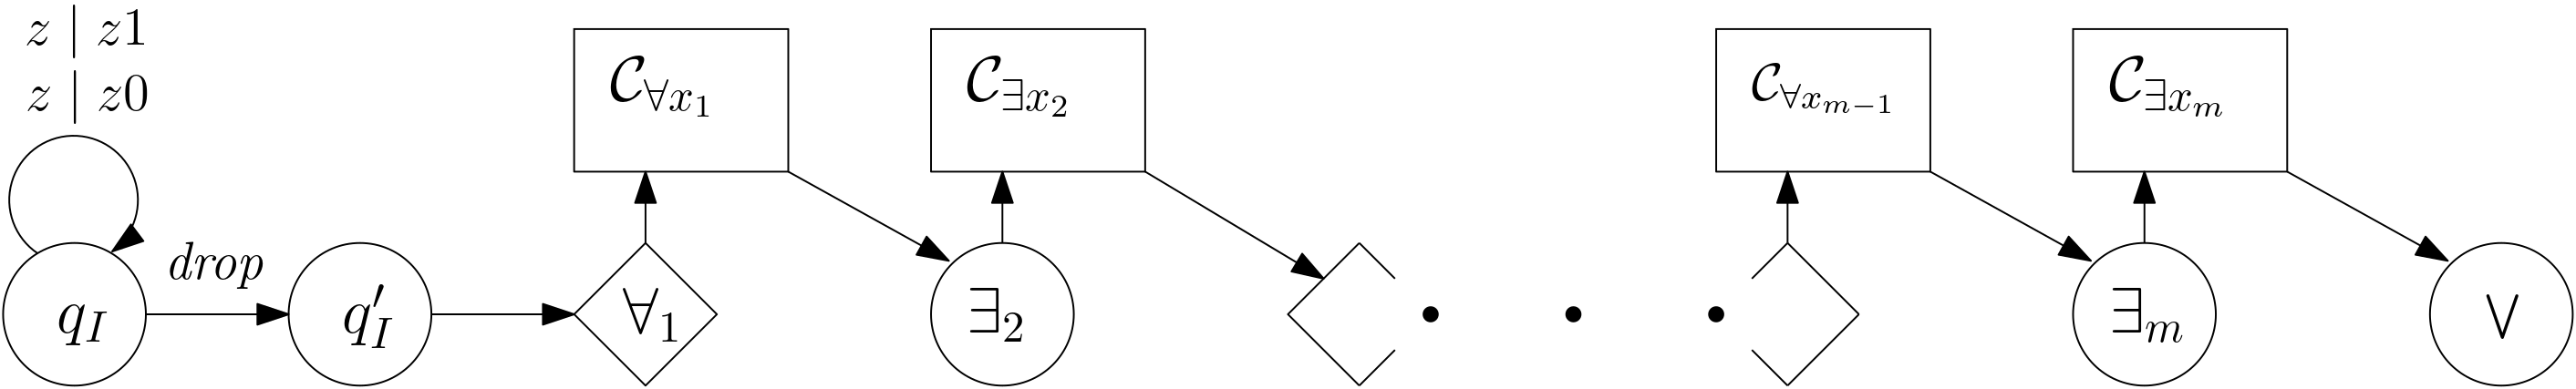
\includegraphics[width=1.01\textwidth]{figures/quantifiers}
	\caption{The begining of the automaton, and thus, of the game, essentially corresponds to a preprocessing steps dealing with the quantifiers. P%layer $0$ add $w$ to the stack, then
	%p
layers take turns %chosing particular
	proving the parameters chosen correspond to prefixes of $w$. Once every variable has been checked%assigned with the dropping of a corresponding pebble
	, players enters the second part of the game.}
		 \label{quantifiers}
	\end{figure}
\end{center}


The first step of the game is to check that the values assigned to the parameters correspond indeed to possible variables, that is, that the values of the parameters are prefixes of $w$. See Figure~\ref{quantifiers} for an illustration of what is happening.
%
% W.l.o.g, we assume $\psi$ to be in disjunctive normal form, that is, that 
%
% $$ \psi = \bigvee_{i \in \N} (\bigwedge_{j \in \N} \psi_{i,j} )$$
%
% where $\psi_{i,j}$ are atomic formula.

Recall $\psi$ is quantifier-free and in disjunctive normal form, i.e.
 $$\phi = \forall x_1 \exists x_2 \forall x_3 \ldots \exists x_k \bigvee_{i=1}^l(\bigwedge_{j=1}^{h_i} \psi_{i,j}(x_1, \ldots, x_k)).$$

Player $0$, being the existential player, chooses one of the conjunctive clauses in $\psi$, essentially claiming to be able to prove it. Then player $1$, the universal player, chooses one of the atomic formulas in the clause to test. The process can be seen in Figure~\ref{DNF}. Testing the atomic formula is the purpose of a gadget $ \C_{\psi_{i,j}}$ built such that player $0$ has a winning strategy in $ \C_{\psi_{i,j}}$ if and only if 
$w$ satisfies $\psi_{i,j}$ if the variables $x_1, \ldots, x_k$ are interpreted by 
$ |\mu(p_1)|-1, \ldots, |\mu(p_k)|-1$ respectively.


\begin{center}
	\begin{figure}
		\hspace{2.4cm}
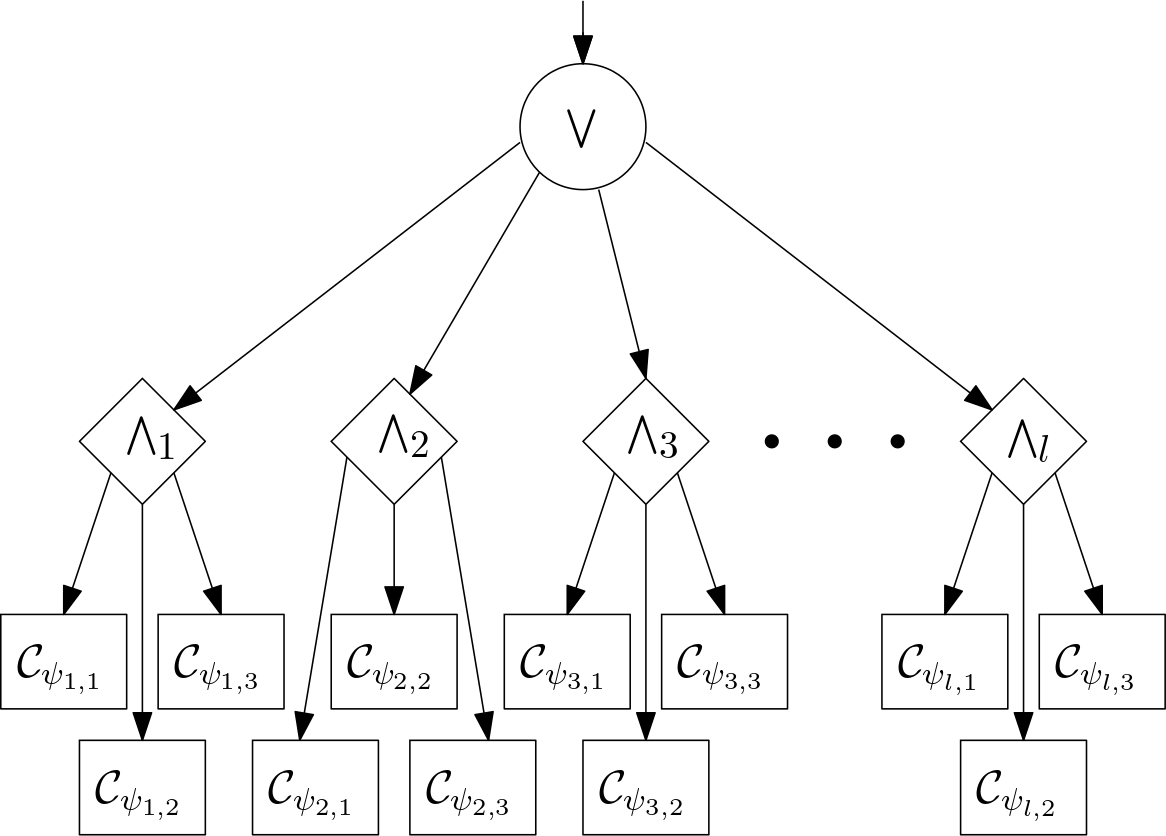
\includegraphics[width=0.6\textwidth]{figures/DNF}
	\caption{Player $0$ chooses which conjunctive clause to test and player $1$ chooses which of the atomic formula in the clause to test. State $\vee$ belongs to player $0$. For $i \in \{1, \ldots, l\}$, state $\wedge_i$ belongs to player $1$.}
		 \label{DNF}
	\end{figure}
\end{center}


Now we need only to describe the gadgets $ \C_{\psi_{i,j}}$. 
The gadget depends on the type of the atomic formula. For a formula checking the letter at the position of a variable $x$, player $0$ goes to the position corresponding to $x$, then checks that the top of the stack
$x$ is the right letter. For one checking that $x = x'$ where $x$ and $x'$ are both variables,
player $0$ goes to the position corresponding to $x$ and checks against the parameter corresponding to $x'$ as well. If the formula is a negation, players exchange their roles. \\






\noindent
Thus we can in polynomial time in $|\phi|$ build a parametric pushdown automaton $\mathcal{Z}$ with $k+1$ parameters, 
 disjoint
unions $Q = Q_0  \biguplus Q_1 $ and $P = P_0 \biguplus P_1$,
and a priority mapping $\Omega$
such that
player $0$ has a 
\iffalse
strategy $\sigma_0$ for the parameter valuation game  such that
for all player $1$ strategies $\sigma_1$ for the parameter valuation game,
player $0$ has a
winning strategy from $q_{init}(\gamma_{init})$ for the reachability condition on
$\mathcal{G}_{(\mathcal{Z}, \mu_{\sigma_0, \sigma_1}, P_0, P_1, Q_0 , Q_1, \Omega)}$ 
\fi
		winning strategy from $\mu_\bot$ in the parity game
		$\mathcal{G} =(A_{(\mathcal{Z}, P_0, P_1, Q_0 , Q_1)}, \win_{\widehat{\Omega}})$ 
if and only if
there exists
%a word $\mathfrak{W} \in \{0,1\}^*$ such that
a word $w \in \{0,1\}^*$ such that
%$\mathfrak{W}  \models \phi $.  \\
$w \models \phi$.
\end{proof}

Then, the nonelementary lower bound follows from Theorem~\ref{FOnonelementary}. 
% Indeed, if there was an elementary function $f$ and an algorithm deciding the  {\sc Parametric pushdown reachability game}  with running time bounded by $f(k)$, where $k$ denotes the size of the input parametric pushdown automaton, then the reduction would lead to a contradiction of the theorem. 


\begin{theorem}

%The problem of 
{\sc Parametric pushdown reachability game} is not in {\sf ELEMENTARY}.

\end{theorem}

As a consequence, %the problem of {\sc Parametric pushdown parity game}
solving parametric pushdown parity games
%and the problem of {\sc Parametric pushdown B\"uchi game}
% are both
is 
 nonelementary too.

\begin{corollary}

%The problem of 
{\sc Parametric pushdown parity game} is not in {\sf ELEMENTARY}.

\end{corollary}

%\subsection{A decidability result from reduction to parity games on automata with pebbles}\label{pebbles}
\section{%A decidability result via r
Reduction to pebble pushdown automata parity games
}\label{pebbles}



% \mh{Motivates the use of pebbles. See pebbles on two-way automata, two-way tree automata, weighted automata, etc.}



% 21. Globerman, N., Harel, D.: Complexity results for two-way and multi-pebble automata and their logics. Theor. Comput. Sci. 169, 161–184 (1996)
%		same as [13] bellow
%
% Engelfriet, J., Hoogeboom, H.J.: Tree-walking pebble automata. In: Karhumäki, J., Maurer, H., Pa ̆un, G., Rozenberg, G. (Eds.) Jewels are Forever, Contributions to Theoretical Computer Science in Honor of Arto Salomaa, pp. 72–83. Springer, Berlin (1999) for tree-walking automata.
%
% @incollection{engelfriet1999tree,
%  title={Tree-walking pebble automata},
%  author={Engelfriet, Joost and Hoogeboom, Hendrik Jan},
%  booktitle={Jewels are forever},
%  pages={72--83},
%  year={1999},
%  publisher={Springer}
%}
% 
%
% Two-way pebble transducers for partial functions and their composition, Joost Engelfriet
%
% Tree-Walking Pebble automata, Joost Engelfriet and Hendrik Jan Hoogeboom 
A pebble automaton is a two-way finite state automaton that uses a fixed, finite number of
pebbles that it can drop on, and lift from 
words, using them as markers.
Pebble automata recognize regular languages only, provided the life times of the pebbles, i.e. the times between dropping a pebble and lifting it again, are properly nested
\cite{globerman1996complexity, engelfriet1999tree}.
Automata with nested pebbles were also introduced
for tree-walking automata. 
It is known that tree-walking automata do not recognize all regular tree languages \cite{bojanczyk2008tree}%, the main trouble being that tree-walking automata get lost rather easily
.
Using pebbles is a remedy against getting lost along a tree, but 
the unrestricted use of pebbles leads to a class of tree languages much larger than the
regular tree languages, in fact to all tree languages in $\NSPACE(log ~ n)$.
Thus, in  both pebble word automata and pebble tree-walking automata, the placement of the pebble follows a strict stack discipline. It is traditional hence to represent syntactically the dropping and lifting of pebbles by operations \textit{lift} and \textit{drop}; a \textit{drop} simply records the current position with a fresh pebble (such a pebble should be available) % and returns to the beginning of the tape, 
and a \textit{lift} pops the last dropped pebble if the current position corresponds to the one recorded by it.




In this section, we extend these ideas to pushdown automata. Instead of using pebbles as markings on their input, pebble pushdown automata have the ability to lift or drop pebbles on their universe of stack contents; a \textit{drop} simply records the current stack content with a fresh pebble (such a pebble should be available) % and returns to the beginning of the tape, 
and a \textit{lift} pops the last dropped pebble 
while requiring that
% assuming
 it was placed on the current node. 
% Thus hierarchicality on the registers works slightly differently from hierarchicality on the pebbles, hierarchicality on the registers being a syntactic property, whereas hierarchicality on the pebbles is a semantical one.
One can think of a pebble as a register that can store a stack content for later comparisons.



We first define more formally our pebble pushdown automaton framework, and then provide a reduction from the problem of solving parametric pushdown parity games to the problem of solving pebble pushdown parity games.



%\subsubsection{Pebble pushdown automata}
\subsection{Pebble pushdown automata}

\newcommand{\ppda}{\mathcal{I}}
% \Denarius
% \vernal
% \mathscr{Z}
% \mathcal{I}
% \pluto
% \capricornus
% \Bumpeq
% \Pfund

An {\em $n$-pebble pushdown automaton} 
is a tuple 
$\ppda = (Q, \Gamma,  R, q_{init}, \gamma_{init}, F)$
where
\begin{itemize}
\item $Q$ is a {\em finite set of  states},
\item $\Gamma$ is a {\em finite stack alphabet},
\item  $R  \subseteq  Q  \times \Gamma \times
		 \{ 0, 1, \ldots n\} \times \mathcal{P}(\{1,\ldots,n\})
		 \times Q  \times (\Op(\Gamma) \cup \{\text{\textit{drop}}, \text{\textit{lift}}\})$ is a {\em finite set of rules},
		 where the fourth element $S$ of a rule $r$ is a subset of 
		$\mathcal{P}(\{1,\ldots,i\})$ where $i$ is the third element of $r$,
		and if the last element is
		$\text{\textit{lift}}$ then we additionally require $i \in S$,
\item $q_{init} \in Q$ is an {\em initial  state}, 
\item $\gamma_{init} \in \Gamma$ is an {\em initial stack symbol}, and
\item $F \subseteq Q$ is a {\em set of final  states}.
\end{itemize}

 
%%%%%%%%%%%%%%%%%%%%%%%%%%%%%%%%%%%%%%%%%%%%%%%%%%%%%%%%%%% 
% \mh{remind the reader what a partial function is}
 
\par\noindent\ignorespacesafterend 
Recall that for \iffalse a partial function $f$ from a set $S$ to a set $X$ 
%is a function defined on a subset $C$ of $S$ (possibly $S$ itself) with output values in $X$, and 
that is defined on a subset $C \subseteq S$
is denoted by
$ f : S \rightharpoonup X $.

For \fi a partial function $ f : S \rightharpoonup X $ (see page~\pageref{partial}), for notational purposes, we consider some element $\bot_X \not\in X$ and 
 associate $f$ with the function returning the 
bottom element $\bot_X$ when $f$ is undefined. Thus we write $(X \biguplus \{ \bot_X \})^S$ for the set of all partial functions from $S$ to $X$, which we here abbreviate as $(X \biguplus \{ \bot \})^S$. 


%%%%%%%%%%%%%%%%%%%%%%%%%%%%%%%%%%%%%%%%%%%%%%%%%%%%%%%%%%%
 
 
% An $i$-configuration of $\ppda$ is an element of
%$ Q\times W^* \times (W^*)^{\{1, \ldots i\}}$.
% By $\Conf_i(\ppda)$ we denote the set of $i$-configurations of $\ppda$.
By $\Conf(\ppda)=Q\times \Gamma^* \times (\Gamma^* \biguplus \{ \bot \})^{\{1, \ldots, n\}}$ we denote the set of
% By $\Conf(\ppda) = \bigcup_{0 \leq i \leq n} \Conf_i(\ppda)$ we denote the set of
{\em configurations} of $\ppda$. As expected, we rather write $q(w, \mu)$ instead of $(q, w, \mu)$.
An {\em$i$-configuration} for $i > 0$ of $\ppda$ is a configuration $q(z,\mu)$ where
$\text{Dom}(\mu) = \{1, \ldots, i\}$, while a $0$-configuration is a configuration 
 $q(z,\mu)$ where $\text{Dom}(\mu)=\emptyset$.



The idea of a transition $(q, a, i, S, q', m) \in R$
is that, if the automaton $\ppda$ is in state $q$ with pebbles $1,\ldots, i$ dropped \---- or without pebble dropped if $i = 0$ \---- with top stack symbol $a$, and stack content which corresponds to the stack contents of the pebbles from $S$ and only these pebbles, then
$\ppda$ goes to state 
$q'$ and makes modifications to the stack or the pebbles according to
$m$. 
% \mh{The set $S$ is used for testing the presence of certain pebbles.}
Note a pebble 
can be lifted only if the stack content which corresponds to the pebble
is the same as the current stack content. 
%$\Dzeta$ $\zeta$ $\Xi$
This is enforced by syntactically requiring
the last pebble dropped $i$ is in the set $S$ used for testing the presence of certain pebbles.

\iffalse
A {\em weak} $n$-pebble pushdown system is an $n$-pebble pushdown system $\ppda = (Q, \Gamma,  \Delta )$ in which $\text{\textit{lift}}$ operations also require the presence of the last pebble dropped, i.e.
for all $(q, a, i, S, q', \text{\textit{lift}}) \in \Delta$, we have $ i \in S $. 
%  is an additionnal restriction $f(i) = wa$ that needs to hold for the application of the $lift$ operation.
{\em Weak $n$-pebble pushdown games} are defined naturally as $n$-pebble pushdown games on 
weak $n$-pebble pushdown systems.

\fi



A {\em pebble set} of $\ppda$ is a set $U \subseteq \{ 1, \ldots, n\}$. For a stack alphabet $\Gamma$, a 
{\em $U \!$-pebble assignment} is a function which maps each $j \in U$ to a word in $ \Gamma^*$.
The $\emptyset$-pebble assignment is denoted by $\mu_{init} :  \{ 1, \ldots, n\} \rightharpoonup  \Gamma^* $ and is the 
%partial function from  $\{ 1, \ldots, n\}$ to $ \Gamma^* $ that
%does not map any $j \in \{ 1, \ldots, n \}$ to an output.
totally undefined function.


\iffalse
For $0 \leq i \leq n$, an {\em $i$-configuration} is a tuple $(q, w, \mu )$, where $w \in \Gamma^*$, $q$ is a state and
$\mu$ a $\{ 1, \ldots , i \}$-pebble assignment. 
We call $w$ the current stack, $q$ the current state and
$\mu$ the current pebble assignment. 
We also write $(q,w, w_{1} , \ldots , w_{i} )$ if 
$\mu(j) = w_j$, for each
$j \leq i$.

The set of configurations is the union of all $i$-configurations for $0 \leq i \leq n$. 
\fi


\begin{samepage}
%\begin{definition}
An $n$-pebble pushdown automaton $\ppda =  (Q, \Gamma,  R, q_{init}, {\gamma_{init}} , F)$ induces 
a transition system  $T_{\ppda} = (\Conf(\ppda), \rightarrow_{\ppda})$ 
 such that
for all $(q, a, i, S, q', m) \in R$, with $a \in \Gamma$,
 for all words $w \in  \Gamma^*$, and for all $\{ 1, \ldots , i \}$-pebble assignments $\mu$ such that $\mu(j) = wa$ 
 %(respectively $\mu(j)= {\gamma_{init}}  $) 
 for each
$j \in S$ 	and
 $\mu(j) \neq wa$ 
 %(resp. $\mu(j) \neq {\gamma_{init}} $) 
 for each $j \in \{ 1, \ldots , i \} \setminus S$,
the following holds
\begin{itemize}
\item if $m \in \Op(\Gamma)$, 
% $(q,wa,\mu) \rightarrow_{\ppda} (q',wm, \mu)$, 
either
\begin{itemize}
\item $ m = \text{\textit{push}}^\gamma$ and $(q,wa,\mu) \rightarrow_{\ppda} (q',wa\gamma, \mu)$,

\item $ m = \text{\textit{pop}}$ and $(q,wa,\mu) \rightarrow_{\ppda} (q',w, \mu)$, or

\item $ m = \text{\textit{skip}}$ and $(q,wa,\mu) \rightarrow_{\ppda} (q',wa, \mu)$,
\end{itemize}
\item if $ m = \text{\textit{drop}}$, 
$(q,wa,\mu) \rightarrow_{\ppda} (q',wa, \mu')$,  
where $\mu'$ is the $\{ 1, \ldots , i, i+1 \}$-pebble assignment such that
$\mu'(j) = \mu(j)$, for each
$j \leq i$, and $\mu'(i+1) = wa$, and
\item if $m = \text{\textit{lift}}$, and $i \in S$, i.e. the last pebble dropped belong of the set of pebble we test the presence of,
$(q,wa,\mu) \rightarrow_{\ppda} (q',wa, \mu')$, 
where $\mu'$ is the $\{ 1, \ldots , i - 1 \}$-pebble assignment such that
$\mu'(j) = \mu(j)$, for each
$j < i$.
\end{itemize}
%\end{definition}
\end{samepage}


\par\noindent\ignorespacesafterend
We are interested in games over pebble pushdown automata, % namely, 
%reachability, B\"uchi, and parity games.
mainly, parity games.

Again, given
a 
%labeled
 transition system, one needs only to provide 
%a mapping $\Omega$ and 
a partition of the set of
configurations 
%$S$ into two sets $S_0$ and $S_1$
 to obtain an arena.
 %
Given a partition of
$Q$ into $Q_0$ and $Q_1$, 
we partition the configurations of
$T_{\ppda}$
into
$\Conf_{\ppda,0}=Q_0\times \Gamma^* \times ( \Gamma^* \biguplus \{ \bot \})^{\{1, \ldots n\}}$
and
$\Conf_{\ppda,1}=Q_1\times  \Gamma^* \times ( \Gamma^* \biguplus \{ \bot \})^{\{1, \ldots n\}}$. 



With these notations in mind one can  define the arena
$$
A_{(\ppda, Q_0 , Q_1)}
=
(\Conf_{\ppda,0}, \Conf_{\ppda,1}, \rightarrow_{\ppda}).$$




As expected, given a 
priority function $\Omega: Q \to \{0, \ldots m\}$,
one naturally 
set the extension of $\Omega$ as
$\overline{\Omega}: \Conf(\ppda) \to \{0, \ldots m\}$
and
$\overline{\Omega}(q, w,\mu) = \Omega(q)$
for all
$w \in  \Gamma^*$
and
$\mu \in ( \Gamma^* \biguplus \{ \bot \})^{\{1, \ldots, n\}}$. \\









Concerning pebble pushdown automata, we are interested in the following decision problem.


\problemx{$n$-pebble pushdown parity game}
{An $n$-pebble pushdown automaton $\ppda= (Q, \Gamma,  R, q_{init}, {\gamma_{init}} , F)$, 
where $Q = Q_0  \biguplus Q_1 $, 
and
a priority mapping $\Omega: Q \to \{0, \ldots m\}$.}
{Does player $0$ have a winning strategy from $q_{init}(\gamma_{init}, \mu_{init})$ for the parity game 
$\mathcal{G}= (A_{(\ppda, Q_0 , Q_1)}, \win_{\overline{\Omega}})$ ?\newline}



% \subsubsection{Reduction from parameters to pebble pushdown automata}
\subsection{From parametric pushdown 
automata 
to pebble pushdown automata
}

We now provide a reduction from the problem of solving parametric pushdown parity games to the problem of solving pebble pushdown parity games. 


\begin{theorem}\label{PPDA reduction}
%The problem of 
{\sc $n$-parametric pushdown parity game} 
is polynomial time reducible to
%the problem of 
{\sc $n$-pebble pushdown parity game}.
\end{theorem}




\begin{proof}[Sketch]


Let us fix some
$n$-parametric pushdown automaton $\mathcal{Z}= (Q, \Gamma, 
P%\{p_1, \ldots, p_n \}
, q_{init}, { \gamma_{init}} , F)$,
 disjoint
union $Q = Q_0  \biguplus Q_1$
and $P = P_0 \biguplus P_1$,
and
some priority function 
$\Omega : Q \times \Gamma^* \times ( \Gamma^* \biguplus \{ \bot \})^R \to [0, m ]$.


We construct
% polynomial time
  an 
 $n$-pebble pushdown automaton $\ppda =(Q', \Gamma,  R', q_{init}', {\gamma_{init}} , F')$,
a 
 disjoint
union $Q' = Q_0'  \biguplus Q_1'$
and a mapping $\Omega' : Q \times  \Gamma'^* \times ( \Gamma'^* \biguplus \{ \bot \})^{\{1, \ldots, n\}} \to \{1, \ldots, m \}$,
such that
 %:
%
player $0$ has a winning strategy from 
$(q'_{init},\gamma_{init}, \mu_{init})$
in
		\iffalse
		for the parity condition on
		$\mathcal{G}_{(\ppda, Q'_0, Q'_1, \Omega')}$.
		\fi
the parity game
$\mathcal{G'}= (A_{(\ppda, Q'_0, Q'_1)}, \win_{\overline{\Omega'}})$
if and only if
player $0$ has a 
		\iffalse
		strategy $\sigma_0$ for the parameter valuation game  such that
		for all player $1$ strategies $\sigma_1$ for the parameter valuation game,
		player $0$ have a
		winning strategy from $q_{init}(\gamma_{init})$ for the parity condition on
		$\mathcal{G}_{(\mathcal{Z}, \mu_{\sigma_0, \sigma_1}, P_0, P_1, Q_0 , Q_1, \Omega)}$. 
		\fi
winning strategy from $\mu_\bot$ in 
the parity game
$\mathcal{G} =(A_{(\mathcal{Z}, P_0, P_1, Q_0 , Q_1)}, \win_{\widehat{\Omega}})$,
where		 
$A_{(\mathcal{Z}, P_0, P_1, Q_0 , Q_1)}$
and
$\widehat{\Omega}$
correspond to the definitions on page~\pageref{PPDA reachability game}.

%
%
%
%


The transition graph of the $n$-pebble pushdown automaton $\ppda$ will simulate the possible transitions graphs 
(one for every 
%total 
parameter assignment)
 of the pushdown automaton with $n$ parameters by using pebbles to represent the parameters. 
The $n$-pebble pushdown automaton will first simulate the 
parameter valuation arena.
Players take turns chosing particular stack contents on which to place pebbles,
using a gadget similar as the one from Figure~\ref{quantifiers}. 
Once every parameter has been assigned with the dropping of a corresponding pebble, 
the pebble assignment $\mu$ is fixed.
%%
%
%
%
%
%
%


Further configurations in the $n$-pebble pushdown automaton then consist of a word representing the status of the stack, a state, and a fixed pebble assignment. For a fixed pebble assignment there is then a one for one correspondance between configurations of the $n$-parametric pushdown 
automaton 
%transition system with assignment $\mu$
and these of the $n$-pebble pushdown automaton. The set of states of the $n$-pebble pushdown automaton apart from the initial gadget is the same as 
the set of states of the $n$-parametric pushdown automaton, and 
so are player $0$ states, player $1$ states and the priority mapping.
\end{proof}




\section{Reduction to higher-order pushdown automata}\label{section HPDA}




Higher-order pushdown automata (HPDA for short) were introduced as a 
generalization of pushdown automata \cite{aho1969nested,Gre70,maslov1976multilevel}. 
% Alfred V. Aho. Nested stack automata. J. ACM, 16(3):383–406, 1969.
% S. Greibach. Full AFL’s and nested iterated substitution. Inf. Control, 16(1):7–35, 1970.
% A.N. Maslov. Multilevel stack automata. Problemy Peredachi Informatsii, 12:55–62, 1976.
A stack of a pushdown automaton is seen as a {\em level $1$ stack}. 
A pushdown automaton of level $2$ (or $2$-HPDA) then works with a stack of level $1$ stacks. 
In addition to the ability to push
and to pop a symbol on the top-most level $1$ stack, an $2$-HPDA can copy or remove the entire topmost level $1$ stack. 
The definition generalizes to any $n \geq 2$, and $n$-HPDA are similarly defined for all level
$n$ as automata working with a stack of level $(n-1)$ stacks.
% HPDA have been extensively studied as language recognizers [Dam82,Eng83].



We recall the definition from \cite{cachat2007complexity} which itself is taken from \cite{knapik2002higher}. We then provide a
reduction from the problem of solving pebble pushdown parity games to the problem of solving
higher-order pushdown parity games.


\subsection{Higher-order pushdown automata}

A {\em level $1$ stack} (or {\em $1$-stack}) over an alphabet $\Gamma$ is 
simply a %word in $\Gamma^*$
	stack over $\Gamma$, i.e. a word  in $\Gamma^*$.
% an arbitrary sequence $w_0 w_1 \ldots w_n $ of elements of $\Gamma$ for some $n \in \N$. 
A  {\em level $n$ stack} (or {\em $n$-stack}) over an alphabet $\Gamma$, for $n \geq 2$, is a 
non-empty sequence
$ \langle s_0 \rangle \langle s_1 \rangle \ldots \langle s_m \rangle$
of
$(n-1)$-stacks over $\Gamma$,
for some $m \in \N$.
The set of $n$-stacks over $\Gamma$ is denoted by $\mathscr{S}_n(\Gamma)$,
or simply $\mathscr{S}_n$ in case the set $\Gamma$ is obvious from context.
The set of all stacks over $\Gamma$ is written $\mathscr{S}(\Gamma) = \bigcup_{n\in \N} \mathscr{S}_n(\Gamma)$.
We define $\epsilon_{1}$ as
$\epsilon \in \Gamma^*$ and we inductively define 
$\epsilon_{n} = \langle \epsilon_{n-1} \rangle$ in $\mathscr{S}_n$ for all $n > 1$.




A {\em higher-order stack operation} is a partial function from $\mathscr{S}(\Gamma)$ 
to $\mathscr{S}(\Gamma)$ which preserves the level of the input (i.e. the image of
an $n$-stack is an $n$-stack for all $n \in \N$). The {\em level } of an operation $op$
is the smallest $n \in \N$ such that $\text{Dom}(op) \cap \mathscr{S}_n \neq \emptyset$. 
The operations 
%we consider
additionally
 respect the hierarchicality of higher-order stacks, i.e. in
a level $n+1$ stack only the topmost level $n$ stack can be accessed. An operation
$op$ of level $n$, applied to a level $n+1$ stack 
$ \langle s_0 \rangle \langle s_1 \rangle \ldots \langle s_m \rangle$
of length $m \in \N$,
thus
returns the output
$ \langle s_0 \rangle \langle s_1 \rangle \ldots \langle op(s_m) \rangle$
if applicable.
The definition for  all levels of stacks greater than $n$ follows the same pattern.


% For all $m \in \N$, 
The following operations can be performed on a $1$-stacks of length $m \in \N$.
% $ w_0 w_1 \ldots w_m \in \Gamma^*$.
\begin{eqnarray*}
&\text{\textit{push}}_1^\gamma( w_0 w_1 \ldots w_m) &=\quad w_0 w_1 \ldots w_m \gamma   \text{ for all } \gamma \in  \Gamma, \\
&\text{\textit{pop}}_1(w_0 w_1 \ldots w_{m-1} w_m ) &=\quad w_0 w_1 \ldots w_{m-1}, \text{ if } m \geq 1\\
&\text{\textit{top}}( w_0 w_1 \ldots w_m ) &=\quad w_m.
\end{eqnarray*}
The operations added at level $n+1$ are the copy of the topmost $n$-stack
and the removal of the topmost $n$-stack.
More formally, if $ \langle s_0 \rangle \langle s_1 \rangle \ldots \langle s_m \rangle$ is a stack of 
level $n > 1$, 
the following operations are possible.
%
\begin{eqnarray*}
&\text{\textit{push}}_n( \langle s_0 \rangle \langle s_1 \rangle \ldots \langle s_m \rangle) &=\quad  \langle s_0 \rangle \langle s_1 \rangle \ldots \langle s_m \rangle \langle s_m \rangle , \\
&\text{\textit{push}}_j( \langle s_0 \rangle \langle s_1 \rangle \ldots \langle s_m \rangle) &=\quad \langle s_0 \rangle, \langle s_1 \rangle \ldots 
\langle \text{\textit{push}}_j(s_m) \rangle,
\text{ if } 2 \leq j < n\\
&\text{\textit{push}}_1^\gamma( \langle s_0 \rangle \langle s_1 \rangle \ldots \langle s_m \rangle) &= \quad
\langle s_0 \rangle \langle s_1 \rangle \ldots 
\langle \text{\textit{push}}_1^\gamma(s_m) \rangle,
\text{ for all } \gamma \in \Gamma,\\
&\text{\textit{pop}}_n( \langle s_0 \rangle \langle s_1 \rangle \ldots \langle s_{m-1} \rangle \langle s_m \rangle) &= \quad
\langle s_0 \rangle \langle s_1 \rangle \ldots \langle s_{m-1} \rangle
,\\
&\text{\textit{pop}}_j( \langle s_0 \rangle \langle s_1 \rangle \ldots \langle s_{m-1} \rangle \langle s_m \rangle) &= \quad
\langle s_0 \rangle \langle s_1 \rangle \ldots \langle s_{m-1} \rangle
\langle \text{\textit{pop}}_j(s_m) \rangle,
\text{ if } 1 \leq j < n\\
&\text{\textit{top}}( \langle s_0 \rangle \langle s_1 \rangle \ldots \langle s_m \rangle) &=\quad
\text{\textit{top}}(s_m).
\end{eqnarray*}
% We omit the stack alphabet $\Gamma$ from 
%The operation $pop_j$ is undefined on a stack whose top stack of level $j$ is empty.
The operations $pop_1$ and $top$ are undefined on a stack whose top $1$-stack is empty.  \\


Given a stack alphabet $\Gamma$ and $n \in \N$, 
we denote by  $\Op_n(\Gamma)$ the {\em base set of $n$-stack operations} as

\begin{itemize}
\item $\text{\textit{push}}_j$ for all $2 \leq j \leq n$,

\item $\text{\textit{push}}_1^\gamma$ for all $\gamma \in \Gamma$,

\item $\text{\textit{pop}}_j$ for all $1 \leq j \leq n$,

\item $\text{\textit{skip}}$, corresponding to the identity function of $\mathscr{S}(\Gamma)$.

\end{itemize}




% \begin{definition}
\begin{samepage}
\par\noindent\ignorespacesafterend
A {\em higher-order pushdown automata of level $n$} (or $n$-HPDA for short) 
is a tuple $\H=(Q, \Gamma, R, q_{init}, \gamma_{init}, F)$,
where 
\begin{itemize}
        \item $Q$ is a non-empty finite {\em set of  states},
        \item $\Gamma$ is a non-empty finite {\em  stack alphabet},
	\item $R\subseteq Q\times \Gamma \times Q \times \Op_n(\Gamma)$ is a finite {\em set of  rules},
        \item $q_{init}$ is the {\em initial  state},
        \item $\gamma_{init} \in \Gamma$ is the {\em %bottom-of-stack
initial stack symbol}, and
	\item $F\subseteq Q$ is a {\em set of final  states}.
		\end{itemize}
\end{samepage}
% \end{definition}

\par\noindent\ignorespacesafterend
By $\Conf(\mathcal{H}) = Q \times \mathscr{S}_n(\Gamma)$
we denote the set of {\em configurations} of an $n$-HPDA $\H$. 
%is a pair $(q, s)$ where $q \in Q$ and $s$ is an $n$-stack over $\Gamma$. 
As usual we abbreviate $(q,s) \in \Conf(\mathcal{H})$ as $q(s)$.



An $n$-HPDA $\H=(Q, \Gamma, R, q_{init}, F)$
induces the transition system $\T_\H = (Conf(\mathcal{H}), \rightarrow_{\mathcal{H}})$
where
for all $q,q'$ in $Q$,
for all $s,s'$ in $\mathscr{S}_n(\Gamma)$,
$q(s) \rightarrow_{\mathcal{H}} q'(s')$ if
there exists some rule
%$(q,\gamma,q',\theta) \in R$
$(q,\gamma,q',op) \in R$
such that
$\text{\textit{top}}(s) = \gamma$
and
%$s' = \theta(s)$.
$s' = op(s)$.




\iffalse
For our constructions it would be simpler to assume that k-HPDS can work
also on stacks of lower levels, in particular on 1-stacks. Of course we can always
simulate a j-stack, for j < k with an k-stack but in the notation it requires some
additional parenthesis that make it less readable.

To define a game on the graph of a HPDA, we assign a player to each control
state, and we consider an initial configuration: a game structure on a HPDS H
is a tuple G = (H, P0 , P1 , s0 ), where P = P0 ⊎ P1 is a partition of the control
states of H, and s0 ∈ Sk . This extends naturally to a partition of the set of
configurations: with the notations of Section 2.1, V0 = P0 × Sk , V1 = P1 × Sk ,
and E is defined above.
\fi

Again we are interested in parity games.
As expected, given an 
 $n$-HPDA $\mathcal{H}$
 and a partition of
$Q$ into $Q_0$ and $Q_1$,
we partition the configurations of
$T_{\mathcal{H}}$
into
$\Conf_{\mathcal{H},0}=Q_0\times \mathscr{S}_n(\Gamma)$
and
$\Conf_{\mathcal{H},1}=Q_1\times\mathscr{S}_n(\Gamma)$.
%
%
With these notations in mind one can define the arena
$$
A_{(\mathcal{H}, Q_0, Q_1)}
=
(\Conf_{\mathcal{H},0}, \Conf_{\mathcal{H},1}, \rightarrow_{\mathcal{H}})$$
\par\noindent\ignorespacesafterend
induced by an $n$-HPDA $\mathcal{H}$ and a partition of its set of states.


As expected, given a 
priority function $\Omega: Q \to [0, m]$,
we naturally extend the function
as follows,
by setting
$\Omega_{\mathscr{S}_n(\Gamma)}: \Conf(\mathcal{H}) \to [0, m]$
and
$\Omega_{\mathscr{S}_n(\Gamma)}(q, s) = \Omega(q)$
for all
$s \in \mathscr{S}_n(\Gamma)$.





Concerning higher-order pushdown automata, we are interested in the following decision problem. 
% \newpage

\begin{samepage}
\problemx{$n$-HPDA parity game}
{An $n$-HPDA $\H= (Q, \Gamma,  R, q_{init}, {\gamma_{init}} , F)$, 
where $Q = Q_0  \biguplus Q_1 $, 
and
a priority mapping $\Omega: Q \to \{0, \ldots m\}$.}
{Does player $0$ have a winning strategy 
from $q_{init}(\text{\textit{push}}_1^{\gamma_{init}}(\epsilon_{n}))$ 
for the parity game 
$\mathcal{G}= (A_{(\H, Q_0 , Q_1)}, \win_{\Omega_{\mathscr{S}_n(\Gamma)}})$ ?\newline}
\end{samepage}

It was shown in \cite{Cach03} that {\sc $n$-HPDA parity game} can
be solved in $n$-$\EXP$. This also gives an $n$-$\EXP$ algorithm for the $\mu$-calculus
model checking over transitions systems induced by  $n$-HPDA.
In \cite{cachat2007complexity} the matching lower bound was showed, even in the case of reachability games,
hence showing $n$-$\EXP$-completeness of {\sc $n$-HPDA parity game}.

\begin{theorem}{\cite{ Cach03, cachat2007complexity}}
{\sc $n$-HPDA parity game} is $n$-$\EXP$-complete.
\end{theorem}


% \subsection{From pebble pushdown automata to higher-order pushdown automata}


In a $2$-HPDA, the operation $\text{\textit{push}}_2$ % allowig to copy a part of the stack, are responsible for the fact the hierarchy of HPDS is strict.
allows to ``copy'' the top level $1$ stack. The current word is hereby stored away and left untouched
until the next operation $\text{\textit{pop}}_2$,
while $\text{\textit{push}}_1$ and $\text{\textit{pop}}_1$ can be performed on the additional ``copy'' in the meantime. This behavior is similar to that of dropping and lifting a pebble. 
The main difference is that there is no operation to test that the ``copy'', after many updates, is again equal to the ``original'', i.e. there is no operation to syntactically test that the two topmost level $1$ stacks are identical.

% But cannot test

\iffalse
In an $n$-HPDA, the operation $\text{\textit{push}}_j$ % allowig to copy a part of the stack, are responsible for the fact the hierarchy of HPDS is strict.
allows to ``copy'' the top stack of level $j$ for all $2 \leq j \leq k$. 
\fi


In \cite{CaWoe03, Woeh05, carayol2006automates} however 
%the authors
Carayol and W\"ohrle
 introduced a variant of $n$-HPDA by extending the 
$\text{\textit{pop}}_j$ operations for $2 \leq j \leq n$ with a built-in equality test. 
For $2 \leq j \leq n$ 
the new operation
$\text{\textit{pop}}_j^=$ has the same effect as $\text{\textit{pop}}_j$, but
can only be applied if the two top level $j$ stacks coincide.
In \cite{carayol2006automates} it is seen as a symmetrical operation in comparison to
$\text{\textit{push}}_j$.\\

A {\em higher-order pushdown automaton with equality pop of level $n$} ($n$-HPDA$^=$ for short) 
is a higher-order pushdown automaton of level $n$ where in
% Instrn
$\Op_n(\Gamma)$
 the operation 
 %popk
 $\text{\textit{pop}}_j$  
  is replaced by 
%  pop=
%k 
$\text{\textit{push}}_j^=$
%for 1 ≤ k ≤ n. 
for $2 \leq j \leq n$.
We denote
this new set of operations by 
% Instr= n
$\Op_n^=(\Gamma)$. 
More formally the new operations $\text{\textit{push}}_j^=$ are defined as
\begin{eqnarray*}
&\text{\textit{pop}}_k^=( \langle s_0 \rangle \langle s_1 \rangle \ldots  \langle s_m \rangle \langle s_m \rangle) &=\quad  \langle s_0 \rangle \langle s_1 \rangle \ldots \langle s_m \rangle , \quad \text{ and }\\
&\text{\textit{pop}}_j^=( \langle s_0 \rangle \langle s_1 \rangle \ldots \langle s_m \rangle) &=\quad \langle s_0 \rangle \langle s_1 \rangle \ldots 
\langle \text{\textit{pop}}_j^=(s_m) \rangle,
\text{ if } 2 \leq j < k. 
\end{eqnarray*}
%
%
%
%
\iffalse
Dans ce sous-paragraphe, nous présentons formellement les automates à pile
de niveau k sur le jeu d'opérations symétriques Opsk et sur le jeu d'opérations
classiques COpsk . Nous donnons à cette occasion un bref historique de la notion
d'automate à pile de piles. Enfin, nous établissons l'équivalence entre les deux
modèles d'automates à chaque niveau en tant qu'accepteurs de langages. Ce résultat a été obtenu dans [CW03] en collaboration ave Stefan Wöhrle. La preuve
complète apparait dans [Wöh05]. Indépendamment, ce résultat a été obtenu dans
[Fra05].
\fi
%
Transition systems induced by higher-order pushdown automata with equality pop of level $n$
are then defined as expected.  
Carayol and W\"ohrle proved \cite{Woeh05, carayol2006automates} that the two models,
namely
higher-order pushdown automata with equality pop of level $n$
and
higher-order pushdown automata of level $n$,
generate the same classes of transition systems.





\begin{theorem}{\cite{Woeh05, carayol2006automates}}
If $\H$ is an $n$-HPDA (resp. $n$-HPDA$^=$) then there
exists an $n$-HPDA$^=$ (resp. $n$-HPDA) $\H'$ such that
$\H$ and $\H'$ %generate the same graph.
induce isomorphic transition systems.
\end{theorem}

\iffalse
\begin{theorem}{\cite{Woeh05, carayol2006automates}}
If $\H$ is an $n$-HPDA  then there
exists an $n$-HPDA$^=$  $\H'$ such that
$\H$ and $\H'$ %generate the same graph.
induce isomorphic transition systems.
\end{theorem}
% Proposition 3.12

\begin{theorem}{\cite{Woeh05, carayol2006automates}}
If $\H$ is an $n$-HPDA$^=$ then there
exists an $n$-HPDA $\H'$ such that
$\H$ and $\H'$ %generate the same graph.
induce isomorphic transition systems.
\end{theorem}

% Proposition 3.18 If A is a higher-order pushdown system with equality pop
% of level n then there exists a higher-order pushdown system B of level n such
% that A and B generate the same graph.
\fi

From $n$-HPDA to $n$-HPDA$^=$ (Proposition 3.12 in \cite{Woeh05}) the proof relies on recreating a correct stack content to simulate higher-order 
$\text{\textit{pop}}$ operations by $\text{\textit{pop}}^=$, essentially ``guessing'' the correct stack content to be able to apply $\text{\textit{pop}}^=$. 
In the other direction (Proposition 3.18 in \cite{Woeh05}), 
the author
enrich the stack alphabet with new symbols stating which 
instructions have to be executed to recreate a
previous stack content. It is proven that such en encoding is possible since
there is 
for every stack $s$ of level $n$
% there is
 a unique shortest sequence of instructions which creates $s$ from
$\epsilon_n$. \\

Defined like {\sc $n$-HPDA parity game}, we write {\sc $n$-HPDA$^=$ parity game}  
in case the input is an $n$-HPDA$^=$ rather than an $n$-HPDA.



The algorithm from \cite{Cach03} actually provides an algorithmic solution to parity games on the graphs of the Caucal hierarchy. 
We skip a formal definition of a graph of level $n$ in the Caucal hierarchy, and refer the reader
to \cite{Cau02mfcs} for more details.
The $n$-$\EXP$ upper bound on $n$-HPDA parity games follows from the fact that every transition system induced by an $n$-HPDA $\H$ is a graph of the Caucal hierarchy \cite{Cach03, Woeh05},
whose vertices are almost in one-to-one correspondence with the configurations of $\H$.
In \cite{Woeh05} the converse direction is proven, i.e. that every graph of level $n$
of the Caucal hierarchy is generated by an $n$-HPDA.  
%
%
In \cite{carayol2006automates}
it is similarly shown that
every transition system induced by an $n$-HPDA$^=$ $\H$ is a graph of the Caucal hierarchy.
%
%
The algorithm from \cite{Cach03} hence lead to a solution for
$n$-HPDA$^=$ parity games as well.



\iffalse
\textcolor{red}{
Now then, because the class of $n$-HPDA$^=$ transitions systems
is the same as
the class of $n$-HPDA transitions systems, we have the following result.
}
\fi

\begin{theorem}\label{HPDA parity game}
{\sc $n$-HPDA$^=$ parity game} is in $n$-$\EXP$.
\end{theorem}





\iffalse
"To show that such an automaton exists we introduce the notion of a weak
popping higher-order pushdown automaton. A weak popping automaton is only
allowed to execute a pop instruction of level $j \geq 2$ if the two top level $j$ stacks
coincide. We skip a formal definition of a weak popping higher-order pushdown
automaton and just mention that even though this automaton model is equipped
with a built-in test on the equality of two stacks of the same level, it is equivalent
to the usual model. All proofs are given in the full version of this article [4]."

Pour pouvoir obtenir une notion pertinente d'ensemble rationnel de piles de
piles, il faut considérer un jeu d'opérations où la destruction inconditionnelle des
piles est remplacée par une version plus symétrique où la dernière pile de niveau ℓ
ne peut être détruite que si elle est égale à la précédente. Nous établissons dans le
paragraphe 4.1 l'équivalence (en temps qu'accepteurs de langages) les automates
à pile définis sur ces deux jeux d'opérations ( f. théorème 4.1.23). Nous montrons,
dans le paragraphe 4.6, le manque de pertinence de la notion de rationalité induite
par le jeu d'opérations classiques et par là même, nous établissons la nécessité de
considérer le jeu d'opérations symétriques.

L'opération de destruction symétrique a été introduite pour des raisons techniques dans 
[CW03] et a été utilisée de manière 
systématique dans [Car05] et
[Fra05]. 
Nous montrerons, dans le sous-paragraphe 4.1.5, que les automates à pile
de piles définis en utilisant les opérations destrk ou les opérations copyk acceptent
les mêmes langages.

Les automates à pile d'ordre supérieur ont été introduits dans les années 70.
Dans [Gre70℄, Greibach attribue l'idée de ces automates à Aho et Ullman. Ces
automates sont aussi définis dans [Mas76℄. Les automates sur COpsk diffèrent
légèrement des automates considérés par ces auteurs et de ceux onsidérés dans
[DG86, Eng91℄. La différence majeure réside dans la définition des piles de piles.
Les piles de niveau k sont des suites non vides de couples formés d'un symbole de
pile et d'une pile de niveau k − 1. Comme remarqué dans [KNU02℄, ces symboles
de pile supplémentaires peuvent être simulés dans le modèle des automates sur
COpsk .

Les langages a eptées par les automates à pile sur COpsk sont onnus sous
le nom de langages k -OI ou de langages indexés de niveau k . La première déno-
mination vient des travaux de Damm [Dam82]

Nous allons maintenant établir que les encodages des opérations simulent bien
les opérations sur les encodages des piles.

Lemme 4.1.21. Pour toute pile s ∈ Stacksk (Γ) et pour tout θ ∈ Opsk ,
[[ θ ]]k ([[ s ]]) =
{
[[ θ(s) ]]		si θ(s) est défini,	
non définie		sinon.


Proposition 4.1.22. Tout langage accepté par un automate à pile sur Opsk est
accepté par un automate à pile sur COpsk .

Démonstration. Soit A = (Γ,Σ,τ,Q,I,F,∆) un automate à pile sur Ops⋆k . Nous
définissons un automate B = (Γ,Σ,τ,Q,I,F,∆B ) où l'ensemble des transitions ∆B
est défini par:
∆B = {(p,x,η,q) | (p,x,θ,q) ∈ ∆ et η ∈ [[ θ ]]k }.
Par le lemme 4.1.21, il suit que pour tout w ∈ (Σ)∗ , p ∈ Q et s ∈ Stacksk (Γ):
w
(q0 , [ ]k ) −→ (p,s)
A
⇔
w
(q0 , [ ]k ) −→ (p,[[ s ]]).

Théorème 4.1.23. Les langages acceptés par les automates à pile sur Opsk et
sur COpsk coïncident.


\fi




\subsection{From pebble pushdown 
automata 
to higher-order pushdown 
automata
}



We use HPDA$^=$ parity games to simulate pebble pushdown automata
parity games.
A similar approach was used in \cite{carayol2006automates} to show that $(n + 2)$-level stack
automata could be used to simulate $n$-pebble alternating two-way word automata.


Let us start by discussing the simulation of the dropping and lifting of a pebble in the case of
a pebble pushdown automaton $\ppda$ with only one pebble.
As long as no pebble is dropped, a $2$-HPDA$^=$ $\H$ can simulate 
the behavior of a pebble pushdown automaton $\ppda$ with a $2$-stack containing a single $1$-stack
on which it performs the same operations $\ppda$ performs on its stack.
When the automaton $\ppda$ is in configuration $q(w)$ and drops a pebble, instead of making a pop or a push, we need
to %go to state $q'$ and word $w$ and 
	store the information that the pebble has been
dropped on $w$.
To simulate the next configuration in such a case, we use 
$\text{\textit{ push}}_2$
to store the information that the pebble has been dropped on the word $w$, leading to the new  $2$-stack
$\langle w \rangle \langle w \rangle$. 
Configurations afterwards have $2$-stacks of length two where the first component remains
$w$ until the pebble is lifted.
Lifting the pebble can be done only at the position the
pebble was dropped, by using $\text{\textit{pop}}^=_2$.
Checking that the node
corresponds to the one where the pebble has been dropped simply makes use of
the composition of $\text{\textit{pop}}^=_2$ and $\text{\textit{push}}_2$.
Checking the absence of the pebble can be done by challenging
the opponent to prove the presence of the pebble.

Now, let us detail the case when there is a second pebble, the construction
for each additional pebble being highly similar, where every additional pebble after
the first one would require the addition of another stack level.
Similarly as before, 
as long as no pebble is dropped, the stack of $\H$ 
is a $3$-stack containing a
single $2$-stack that contains a single $1$-stack.
To simulate configurations in the case one pebble have been dropped, the stack contains a single
 $2$-stack of the form $\langle w_1 \rangle \langle w \rangle$.
In the case the two pebbles have been dropped, 
the stack is of the form $ \langle \langle w_1 \rangle \langle w_2 \rangle \rangle
\langle \langle w_1 \rangle \langle w \rangle \rangle$. 



Intuitively speaking, $w_1$ is, as before, the position where the first pebble is
placed, and $w_2$ is where the second pebble is placed. Dropping pebbles like this
again involves the cloning operation, only, each pebble operates at a different 
stack level: thus, dropping the first pebble will use $\text{\textit{push}}_2$
and dropping the second pebble will use $\text{\textit{push}}_3$. Knowing the number of pebbles dropped can be done by 
keeping track using the states of $\H$.
Lifting or
checking for the presence 
(or absence) 
of the pebbles functions on a similar
basis as before. Checking the presence of the first pebble uses 
operation $\text{\textit{pop}}^=_2$ followed by $\text{\textit{push}}_2$,
while checking the presence of the second pebble uses 
operation $\text{\textit{pop}}^=_3$ followed by $\text{\textit{push}}_3$.
Lifting the first pebble uses $\text{\textit{pop}}^=_2$, but
check first that the second pebble has already been lifted.
Lifting the second pebble simply uses $\text{\textit{pop}}^=_3$.


By expanding this reasoning inductively, we conclude that given $n \in N$, and
given an $n$-pebble pushdown automaton 
$\ppda = (Q, \Gamma, R, q_{init}, \gamma_{init}, F)$, where $Q= Q_0 \biguplus Q_1$,
one can compute an $(n+1)$-HPDA 
$\H = (Q', \Gamma, R', q_{init}', \gamma_{init}', F')$  where $Q'= Q_0' \biguplus Q_1'$, 
such 
that 
player $0$ has a winning strategy from $q'_{init}(\text{\textit{push}}_1^{\gamma_{init}'}(\epsilon_{n}))$ in $A_{(\H,Q'_0,Q'_1)}$ 
if
and only if
player $0$ has a winning strategy from $q(\gamma_{init},\mu_{init})$ in $A_{(\ppda,Q_0,Q_1)}$. 
Hence the following reduction.

\begin{theorem} 
{\sc $n$-pebble pushdown parity game} is polynomial time reducible
to {\sc $(n+1)$-HPDA$^=$ parity game}.
\end{theorem}

The reduction implies decidability of pebble pushdown automata parity game. Furthermore,
by Theorem~\ref{HPDA parity game}, it implies the following complexity result.


\begin{theorem}
{\sc $n$-pebble pushdown automata parity game} is in $(n+1)$-$\EXP$.
\end{theorem}

Finally, the following complexity result is due the above and Theorem~\ref{PPDA reduction}.

\begin{corollary}
{\sc $n$-parametric pushdown automata parity game} is in $(n+1)$-$\EXP$.
\end{corollary}





































% \subsection{Discussion and open problems}
\section{Discussion and open problems}\label{discuss ppda}

In this section we have shown that
deciding
the winner of a parametric pushdown parity game or reachability game is nonelementary in general, but
decidable and in $(n+1)$-$\NEXP$ when the number $n$ of parameters is fixed.

	For the lower bound
we reduced the $\FO$ satisfiability problem on words \---- known to be nonelementary
from \cite{Sto74} \---- to the
problem of deciding whether player $0$ has a winning strategy for a parametric pushdown reachability game.

	For the decidability upper bound, we  used
	pebble pushdown parity games
	to solve 
	parametric pushdown parity games, and 
	 higher-order pushdown parity games to solve pebble pushdown parity games.
 Since solving parity games on higher-order pushdown automata with level $n$ stack is $n$-$\EXP$-complete \cite{ Cach03, cachat2007complexity}, this provides an $(n+1)$-$\EXP$ upper bound for solving parametric parity games on parametric pushdown automata with $n$ parameters.



% \mh{question ofreducing PATWA to pebble pushdown is kinda easy, bot now other question: reducing pebble pushdown to parametric pushdown, doable or not ? since register have only 3r values they can 'remember' maybe it can be shown something along theses lines for pebble pushdown idk}




 Since a particular case of pushdown automata consists in one-counter automata, extensions of automata with a counter generally inherit known upper bounds on pushdown automata. 
This however is not the case in
the parametric extensions considered in this thesis, as parametric updates
% in PTOCA
 are not trivially handled by our PPDA model, i.e. a PPDA over a unary alphabet plus a bottom-of-stack symbol is not trivially a PTOCA nor a POCA. 
For solving parametric pushdown parity games, on the other hand, we introduced the notion of pebble pushdown parity games, and
pebble pushdown automata over unary alphabet plus a bottom-of-stack symbol
can be seen as a form of one-counter automata extended with pebbles. 
A pebble one-counter automata is then a one-counter automata that
can use a set of pebbles as markings on the set of non-negative integers, with a 
$\text{\textit{drop}}$ recording the current counter value, and a 
$\text{\textit{lift}}$ poping the last dropped
pebble while requiring that the current counter value 
corresponds to the one from the last dropped pebble.
%
%Hence, u
Unlike for parametric extensions, 
decidability of 
what should be called
pebble one-counter parity games follows from
decidability of pebble pushdown parity games. 
We believe it natural to study such a pebble one-counter automata model
on its own.
In particular we believe that the question of whether or not
solving pebble one-counter reachability games is nonelementary is worth investigating.
% It may very well be the case that the hierarchy collapses instead, at level e.g. 2 or 3.


Of note is that reachability games and parity games are 
not the only problems one can consider, as one can
also explore the complexity of reachability itself. 
In particular
one can 
% ask whether or not the parametric pushdown automata model described in this section  admits effective preservation of regularity.
study the precise complexity of the
{\sc $n$-PPDA reachability} problem.
Since reachability can be viewed as a reachability game, we know that
{\sc $n$-PPDA reachability} is decidable in $(n+1)$-$\EXP$, 
but the precise complexity of the problem remains unknown.
We are furthermore convinced that it is worthwhile to investigate further comparisons between parametric pushdown automata, pebble pushdown automata, 
%pebble alternating tree automata 
and register pushdown automata, especially since the latter have been shown to only really ``remember'' at most  $3r$ data values, where $r$ is the number of registers. 




% \newpage
